% ------------------------------------------
%  MASTER THESIS DISSERTATION
% ------------------------------------------
% Author:
%
% Advisors:
%
% ------------------------------------------
\documentclass[10pt,twoside,openright,a4paper]{report}
\usepackage[utf8]{inputenc}

% Set document margins to 1in in all sides
\usepackage[margin=2.5cm]{geometry}
% Line spacing package
\usepackage{graphicx, helvet, hyperref, setspace}
\usepackage[portuguese,english]{babel}
\usepackage[nomain, acronym, toc]{glossaries}
% Extra stuff file
% This file is included before begin{document} environment
% Use this to include extra packages and define your own commands
% This way, you can easily grab a most recent version
% of dissertation.tex file from the original repo

\usepackage{epstopdf}

% Built the glossary when the main file is built.
\makeglossaries
% Set main font to Arial
\renewcommand{\familydefault}{\sfdefault}
% Define keywords macro
\providecommand{\keywords}[1]{\textbf{Keywords:} #1}
% Define "palavras-chave" macro
\providecommand{\palavrasChave}[1]{\textbf{Palavras-Chave:} #1}
% Define the NewPage macro
\newcommand*\NewPage{\newpage\null\thispagestyle{empty}\cleardoublepage}
% Abstract-en page numbering
\newcommand {\abstractEnglishPageNumber} {\thispagestyle{plain}\setcounter{page}{\abstractEnglishPage}}
% Abstract-pt page numbering
\newcommand {\abstractPortuguesePageNumber} {\thispagestyle{plain}\setcounter{page}{\abstractPortuguesePage}}
% Section numbering depth
\setcounter{secnumdepth}{3}
% Table of contents depth
\setcounter{tocdepth}{3}
% Set line spacing to 1.5cm
\onehalfspacing
% Page numbering
\pagestyle{plain}

% Glossary-File
% Glossary Definition

\newglossaryentry{MSc}{name={MSc}, description={Masters degree in the area of Science.}}

%\newglossaryentry{IST}{name={IST}, description={Instituto Superior T\'ecnico}}
%\newglossaryentry{IoT}{name={IoT}, description={Internet of Things}}
%\newglossaryentry{IdC}{name={IdC}, description={Internet das Coisas}}
%\newglossaryentry{MQTT}{name={MQTT}, description={Message Queue Telemetry Transport}}
%\newglossaryentry{MQTT-SN}{name={MQTT-SN}, description={Message Queue Telemetry Transport for Sensor Networks}}
%\newglossaryentry{CoAP}{name={CoAP}, description={Constrained Application Protocol}}
%\newglossaryentry{HTTP}{name={HTTP}, description={Hypertext Transfer Protocol}}
%\newglossaryentry{TLS}{name={TLS}, description={Transport Layer Security}}
%\newglossaryentry{DTLS}{name={DTLS}, description={Datagram Transport Layer Security}}
%\newglossaryentry{WWW}{name={WWW}, description={World Wide Web}}
%\newglossaryentry{MTU}{name={MTU}, description={Maximum Transmission Unit}}
%\newglossaryentry{TCP}{name={TCP}, description={Transmission Control Protocol}}
%\newglossaryentry{REST}{name={REST}, description={REpresentational State Transfer}}
%\newglossaryentry{UDP}{name={UDP}, description={User Datagram Protocol}}
%\newglossaryentry{URIs}{name={URIs}, description={Universal Resource Identifiers}}
%\newglossaryentry{M2M}{name={M2M}, description={Machine to Machine}}
%\newglossaryentry{QoS}{name={QoS}, description={Quality of Service}}
%\newglossaryentry{WLAN}{name={WLAN}, description={Wireless Local Area Networks}}
%\newglossaryentry{WPAN}{name={WPAN}, description={Wireless Private Area Networks}}
%\newglossaryentry{LR-WPAN}{name={LR-WPAN}, description={Low-Rate Wireless Private Area Networks}}
%\newglossaryentry{MAC}{name={MAC}, description={Medium Access Control}}
%\newglossaryentry{FFD}{name={FFD}, description={Full Function Device}}
%\newglossaryentry{RFD}{name={RFD}, description={Reduced Function Device}}
%\newglossaryentry{IETF}{name={IETF}, description={Internet Engineering Task Force}}
%\newglossaryentry{DoS}{name={DoS}, description={Denial of Service}}
%\newglossaryentry{DODAG}{name={DODAG}, description={Destination Oriented Directed Acyclic Graph}}
%\newglossaryentry{DIO}{name={DIO}, description={DODAG Information Objects}}
%\newglossaryentry{DAO}{name={DAO}, description={Destination Advertisement Objects}}
%\newglossaryentry{DIS}{name={DIS}, description={DODAG Information Solicitation}}
%\newglossaryentry{RFID}{name={RFID}, description={Radio Frequency Identification}}
%\newglossaryentry{ACL}{name={ACL}, description={Access Control List}}
%\newglossaryentry{6LoWPAN}{name={6LoWPAN}, description={IPv6 over Low power Wireless Personal Area Networks}}
%\newglossaryentry{RPL}{name={RPL}, description={Routing Protocol for Low-Power and Lossy Networks}}
%\newglossaryentry{CA}{name={CA}, description={Certificate Authority}}
%\newglossaryentry{CSDS}{name={CSDS}, description={\gls{CoAP} Service Discovery Server}}
%\newglossaryentry{RDC}{name={RDC}, description={Radio Duty Cycling}}
%\newglossaryentry{LLSec}{name={LLSec}, description={Link-Layer Security}}
%\newglossaryentry{AES}{name={AES}, description={Advanced Encryption Standard}}
%\newglossaryentry{CCM}{name={CCM}, description={Counter with CBC-MAC}}
%\newglossaryentry{MIC}{name={MIC}, description={Message Integrity Code}}
%\newglossaryentry{RAM}{name={RAM}, description={Random-Access Memory}}
%\newglossaryentry{OSI}{name={OSI}, description={Open Systems Interconnection}}
% Acronym-File
% Acronym Definition

\newacronym{IST}{IST}{Instituto Superior T\'ecnico}
\newacronym{IoT}{IoT}{Internet of Things}
\newacronym{MQTT}{MQTT}{Message Queue Telemetry Transport}
\newacronym{MQTT-SN}{MQTT-SN}{Message Queue Telemetry Transport for Sensor Networks}
\newacronym{CoAP}{CoAP}{Constrained Application Protocol}
\newacronym{HTTP}{HTTP}{Hypertext Transfer Protocol}
\newacronym{TLS}{TLS}{Transport Layer Security}
\newacronym{DTLS}{DTLS}{Datagram Transport Layer Security}
\newacronym{WWW}{WWW}{World Wide Web}
\newacronym{MTU}{MTU}{Maximum Transmission Unit}
\newacronym{TCP}{TCP}{Transmission Control Protocol}
\newacronym{REST}{REST}{REpresentational State Transfer}
\newacronym{UDP}{UDP}{User Datagram Protocol}
\newacronym{URIs}{URIs}{Uniform Resource Identifiers}
\newacronym{M2M}{M2M}{Machine to Machine}
\newacronym{QoS}{QoS}{Quality of Service}
\newacronym{WLAN}{WLAN}{Wireless Local Area Networks}
\newacronym{WPAN}{WPAN}{Wireless Private Area Networks}
\newacronym{LR-WPAN}{LR-WPAN}{Low-Rate Wireless Private Area Networks}
\newacronym{MAC}{MAC}{Medium Access Control}
\newacronym{FFD}{FFD}{Full Function Device}
\newacronym{RFD}{RFD}{Reduced Function Device}
\newacronym{IETF}{IETF}{Internet Engineering Task Force}
\newacronym{DoS}{DoS}{Denial of Service}
\newacronym{DODAG}{DODAG}{Destination Oriented Directed Acyclic Graph}
\newacronym{DIO}{DIO}{DODAG Information Objects}
\newacronym{DAO}{DAO}{Destination Advertisement Objects}
\newacronym{DIS}{DIS}{DODAG Information Solicitation}
\newacronym{RFID}{RFID}{Radio Frequency Identification}
\newacronym{ACL}{ACL}{Access Control List}
\newacronym{6LoWPAN}{6LoWPAN}{IPv6 over Low power Wireless Personal Area Networks}
\newacronym{RPL}{RPL}{Routing Protocol for Low-Power and Lossy Networks}
\newacronym{CA}{CA}{Certificate Authority}
\newacronym{CSDS}{CSDS}{\gls{CoAP} Service Discovery Server}
\newacronym{RDC}{RDC}{Radio Duty Cycling}
\newacronym{LLSec}{LLSec}{Link-Layer Security}
\newacronym{AES}{AES}{Advanced Encryption Standard}
\newacronym{CCM}{CCM}{Counter with CBC-MAC}
\newacronym{MIC}{MIC}{Message Integrity Code}
\newacronym{RAM}{RAM}{Random-Access Memory}
\newacronym{OSI}{OSI}{Open Systems Interconnection}
\newacronym{IdC}{IdC}{Internet das Coisas}
\newacronym{CETIC}{CETIC}{Centre d’Excellence en Technologies de l’Information et de la Communication}

\glsaddall

% ------------------------------------------
% MASTER THESIS DISSERTATION
% ------------------------------------------

\begin{document}
\pagenumbering{gobble}% Remove page numbers (and reset to 1)
\clearpage
\thispagestyle{empty}
%!TEX root = ./dissertation.tex

% Dissertation basic information
\newcommand {\Title} {Power Aware Security Protocols\\for the Internet of Things}
\newcommand {\Subtitle} {My Subtitle}
\newcommand {\StudentName} {Tiago Miguel Correia Diogo}
\newcommand {\DegreeName} {Information Systems and Computer Engineering}
\newcommand {\Supervisors} {{\large Prof./Dr. Lorem Ipsum}}

% Include or not include acknowledgments
\def \includeAcknowledgments{1}

% Include or not include glossary
\def \includeGlossary{1}

% Examination Committee
\newcommand {\Advisor} {{\large Prof./Dr. Miguel Pardal}}
\newcommand {\CoAdvisor} {{\large Prof./Dr. Co Advisor}}

% After the thesis defense
\newcommand {\CommitteeMembers} {
{\large Prof./Dr. Lorem Ipsum}\\
{\large Prof./Dr. Lorem Ipsum}
}
\newcommand {\Chairperson} {{\large Prof./Dr. Lorem Ipsum}}

% Is final version (will include Committee Members information)
\def \IsFinalVersion{1}

% Date
\newcommand {\Month} {October}
\newcommand {\Year} {2016}

% Acknowledgments page number
\def \acknowledgmentsPage{1}

% Abstract-en page numbering
\def \abstractEnglishPage{3}

% Abstract-pt page number
\def \abstractPortuguesePage{5}

% You had a co-advisor:
\def \HasCoAdvisor{0}

% Logo Spacing Variables
\def \finalLogoSpacing{2.0cm}
\def \draftLogoSpacing{2.0cm}

% Advisors Spacing Variables
\def \finalAdvisorsSpacing{1.0cm}
\def \draftAdvisorsSpacing{10.0cm}

% Date Spacing Variable
\def \dateSpacing{5.0cm}

% You can define your own variables here


%!TEX root = ./dissertation.tex

% ---------------------------------------------------------
%   MASTER THESIS DISSERTATION COVER
% ---------------------------------------------------------
\begin{titlepage}
% ---------------------------------------------------------
%  INSTITUTION LOGO
% ---------------------------------------------------------

\includegraphics[width=5cm]{images/ist_logo}~\\
%
\if\IsFinalVersion 1
  \vspace*{\finalLogoSpacing}
\else
  \vspace*{\draftLogoSpacing}
\fi

\begin{center}
% ---------------------------------------------------------
%  MASTER THESIS DISSERTATION TITLE
% ---------------------------------------------------------
{\LARGE \textbf{\Title}}\\[1.0cm]
% ---------------------------------------------------------
%  MASTER THESIS DISSERTATION SUBTITLE
% ---------------------------------------------------------
%{\Large \Subtitle}\\[1.0cm]
% ---------------------------------------------------------
%  AUTHOR NAME (FULL)
% ---------------------------------------------------------
{\Large \textbf{\StudentName}}\\[1.0cm]
% ---------------------------------------------------------
%  DISSERTATION DEGREE
% -----------------------------------------------------------------
{\large Thesis to obtain the Master of Science Degree in}\\[1.0cm]
% -----------------------------------------------------------------
%  COURSE NAME
% -----------------------------------------------------------------
{\LARGE \textbf{\DegreeName}}\\[1.0cm]

% -----------------------------------------------------------------
%  ADVISORS NAME
% ---------------------------------------------------------
\begin{minipage}[t]{.4\textwidth}
  \center
  \begin{flushright}
    {\large Supervisors:~~}
  \end{flushright}
\end{minipage}%
\begin{minipage}[t]{.6\textwidth}
  \center
  \begin{flushleft}
    {\Supervisors}
  \end{flushleft}
\end{minipage}\\
%
\if\IsFinalVersion 1
  \vspace*{\finalAdvisorsSpacing}
\else
  \vspace*{\draftAdvisorsSpacing}
\fi
% ---------------------------------------------------------
%  JURI NAMES:
%  - PRESIDENT
%  - ADVISOR
%  - VOGALS
% ---------------------------------------------------------
%
\if\IsFinalVersion 1
%
\begin{minipage}[t]{1\textwidth}
  \center
  {\Large \textbf{Examination Committee}}\\[.25cm]
  {\large Chairperson: \Chairperson}\\
  {\large Supervisor: \Advisor}\\
  {\large Member of the Committee: \CommitteeMembers}
\end{minipage}\\[1.0cm]
%
\fi
%

\if\IsFinalVersion 1
 \vspace*{\dateSpacing}
\fi

% ---------------------------------------------------------
%  DATE (MONTH AND YEAR)
% ---------------------------------------------------------
{\Large \textbf{\Month\:\Year}}\\
\end{center}
\end{titlepage}

\NewPage

\pagenumbering{roman}

\if\includeAcknowledgments 1
%!TEX root = ../dissertation.tex

% Acknowledgments: This one is optional
\chapter*{Acknowledgments}
% Thanks to everyone and bla bla bla

\NewPage
\fi

%!TEX root = ../dissertation.tex

\begin{otherlanguage}{english}
\begin{abstract}
% Set the page style to show the page number
\thispagestyle{plain}
\abstractEnglishPageNumber


The \gls{IoT} and its vision of connecting every device to one another and to the Internet presents an opportunity to create large information sharing networks. However, intruders can capture and take advantage of the \gls{IoT} devices' constrained nature to disrupt these networks and launch a wide range of attacks on its nodes. In our work we address this issue from a power-aware perspective, identifying best relation between security and resource consumption. To achieve this objective we do a thorough analysis of the existing protocols, attacks and mitigation strategies, combining that information into our proposed bootstrapping and network management system -- AutoStrap -- evaluated on a Smart Campus scenario. Furthermore, we perform energy, space and time profiling of the network devices to endow future users with the knowledge of what kind of physical resources to deploy based on the proposed application security level.

% Keywords
\begin{flushleft}

\keywords{Internet of Things, Power-Aware Security, Secure Bootstrapping, CoAP, MQTT, 6LoWPAN, RPL, IEEE 802.15.4}

\end{flushleft}

\end{abstract}
\end{otherlanguage}

\NewPage
%!TEX root = ../dissertation.tex

\begin{otherlanguage}{portuguese}
\begin{abstract}
\abstractPortuguesePageNumber

A \gls{IdC} e a sua visão de ligar todos os dispositivos entre sí e à Internet apresenta-se como uma oportunidade para criar grandes redes de captura e partilha de informação. No entanto, instrusos podem debilitar e capturar estas redes aproveitando-se dos seus limitados recursos por lançar uma larga gama de ataques aos seus elementos. No nosso trabalho abordamos este problema numa perspectiva energética, com o objectivo de encontrar a melhor relação entre segurança e consumo energético. Para atingir este objectivo, realizámos uma análise extensiva aos protocolos, ataques e estratégias de mitigação existentes, combinando essa informação no nosso sistema de gestão e arranque seguro de redes -- AutoStrap -- avaliado num cenário SmartCampus. Ademais, conduzimos medições ao nível do espaço utilizado e recursos consumidos para entender quais os recursos fisicos necessários para este tipo de aplicações.

% Keywords
\begin{flushleft}

\palavrasChave{Internet das Coisas, Segurança Energéticamente Ponderada, Aranque Seguro, CoAP, MQTT, 6LoWPAN, RPL, IEEE 802.15.4}

\end{flushleft}

\end{abstract}
\end{otherlanguage}

\NewPage

% Table of contents
\tableofcontents
% A new page is necessary only if table of contents has an odd number of pages
\NewPage

% List of tables
\addcontentsline{toc}{chapter}{\listtablename}
\listoftables
% A new page is necessary only if list of tables has an odd number of pages
\NewPage

% List of figures
\addcontentsline{toc}{chapter}{\listfigurename}
\listoffigures
% A new page is necessary only if list of figures has an odd number of pages
\NewPage

% List of acronyms
\printglossary[type=\acronymtype]

\pagenumbering{arabic}% Arabic page numbers (and reset to 1)

%!TEX root = ../dissertation.tex

% Entry point for chapters
% In this file you define the order
% in which the chapters are included

% Chapters
%!TEX root = ../dissertation.tex

\chapter{Introduction}
\label{chapter:introduction}
The Internet of Things \gls{IoT} can be seen as a web of interconnected devices that go from everyday wearable objects into fully deployed sensor networks. Despite the huge variety and characteristics of these devices, one thing that they all have in common is the constrained nature that they are built upon. In order to enable the massive deployment to be expected in the near future,\footnote{http://blogs.wsj.com/cio/2015/06/02/internet-of-things-market-to-reach-1-7-trillion-by-2020-idc/} \gls{IoT} devices must be accessible and affordable, capable of operating under lossy wireless networks while being battery powered. This poses a challenge to current Internet protocols since the assumptions regarding the devices' capabilities and objectives do not hold true.\\ To allow the \gls{IoT} vision to come forward, several new protocols have been developed across the OSI layers, each addressing and tackling the challenges involved in trying to keep the quality and assurances of stronger, more expensive protocols, on constrained systems. After being thoroughly analysed, these protocols have been selected and grouped in a power-efficient stack, establishing a base line for power consumption.
Additionally, major attention has been given to information security because for both corporations and individuals, the interconnection of the devices around us can provide information about our choices and whereabouts, therefore leaking corporate information or simply reducing our individual privacy \cite{Ukil2015}. Thus, the focus moved towards adding mechanism to ensure authentication, confidentiality and integrity of the transmitted information by securing the communication channel. In order to understand the cost of adding these mechanisms, additional experiments have been performed so that the added power consumption can be measured, profiled and documented, enabling the finding of the best parameters and requirements for a desired level of security.\\

TODO: não tive inspiração suficiente, ainda, para escrever um paragrafo que diga que construimos uma solução assente num cenário smart campus porque é um bom modelo para testarmos o sistema e obtermos medições interessantes, e que também foi dado grande foco na facilidade de uso e monitorização do sistema, permiting a qualquer um sem conhecimentos técnicos fazer deploy da rede de sensores e monitorizar os valores reportados

\section{Document Roadmap}

In this document we start by analysing the state-of-the-art in Section \ref{sec:related_work}. This includes the selection of the most adequate protocol stack for our necessities in Section \ref{sec:protocol_analysis}, an overview of the existing attacks and mitigation strategies in Section \ref{sec:attack_analysis} and a summary of the existing solutions regarding secure insertion of new nodes in an existing network in Section \ref{sec:secure_bootstrapping}. All this knowledge will be integrated into our proposed solution defined in Section \ref{sec:proposed_solution}. Section \ref{sec:work_evaluation} defines how our work will be tested and evaluated so that a power-aware perspective can be achieved. Section \ref{sec:work_planning} states how the development of our solution will unwind over the next months and finally, Section \ref{sec:conclusion} presents the conclusion of this document.
%!TEX root = ../dissertation.tex

\chapter{Environment Overview}
\label{sec:network_overview}
There are many applicability domains and different methods for creating \gls{IoT} networks. 
Some provide direct connectivity of nodes to the Internet while others provide a common gateway for interfacing with external networks. 
In our work, we focus on scenarios where network nodes are not directly connected to the Internet and require additional network components for proper communication as depicted in Figure \ref{fig:net_overview}.

\begin{figure}[h]
  \centering
  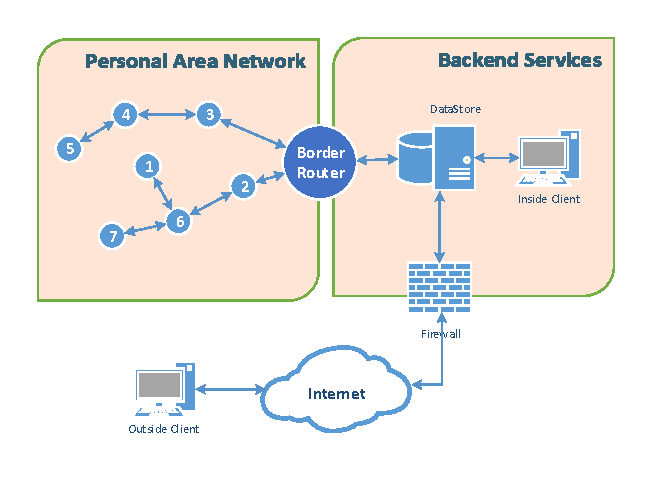
\includegraphics[width=0.8\linewidth]{figures/Network_Overview.pdf}
  \caption{IoT Network Overview.}
  \label{fig:net_overview}
\end{figure}

In this type of architectures, the sensing or actuating nodes belong to a very constrained network with specific protocols and header compression mechanisms, requiring an interface device -- the border router -- in order to communicate with external networks.
After reaching the external network, incoming messages are processed to convert sensor data into useful information which is then stored or used to trigger events. 
This information can then be accessed by users either on the same network or by making requests through the Internet. 

This type of deployment could be used, for example, in a home intrusion system or in a factory monitoring system. 
In the home intrusion system scenario, the network nodes would create a sensor network that propagates events in the case of an intrusion and the additional infrastructure would be in charge of receiving these events and notifying the police authorities. 
In the factory monitoring system scenario, the network nodes would create a sensor network that would be permanently reporting up-to-date readings of machinery control values like: temperature, pressure and power; 
and the additional infrastructure would in charge of supplying this information to a dashboard for the factory workers. 
If an attacker could disable these systems, he could then 
%rob the house or 
cause an emergency shut-down of the factory machinery due to lack of control over the working conditions. 
These are real concerns backed by a range of attacks that focuses on disabling \gls{IoT} networks by placing the nodes offline. These attacks are presented in the following Section.
%TEX root = ../dissertation.tex

\chapter{Related Work}
\label{chapter:related_work}

\section{Protocol Analysis and Selection}
\label{sec:protocol_analysis}

\paragraph{}
There are many alternatives and some proposed standards when it comes to choosing a protocol stack for \gls{IoT} communications. The decision must be based on the particularities of the devices to be used and the objective of the application itself, however a thorough analysis of the existing solutions is a proper way to unveil the strong and weak points of each protocol providing a good basis for an informed decision. A recent survey (January 2015) \cite{Al-Fuqaha2015} of \gls{IoT} enabling technologies, protocols and applications was the starting point for the analysis to follow. The presentation of the available protocols and solutions will follow a bottom-up approach, starting from the data link and physical layer all the way up until the application layer. In particular, the session layer will be left to the end since securing the channel is an optional feature and will be addressed after the application level protocols are properly examined.

\subsection{Data Link and Physical Layer}

\paragraph{}
The first requirement for the physical layer of the \gls{IoT} is the use of wireless radios. These should aim for simplicity, low-power and low-cost communications. While wireless communication is widespread and can be found from homes to airports, the type of radio commonly used, known as Wi-Fi, uses a high amount of power causing concerns for battery life. In the next paragraphs, an overview of Wi-Fi (IEEE 802.11) is given with the objective of comparing it with the IEEE 802.15.4, a protocol that aims to address these issues.

\paragraph{\textbf{IEEE 802.11}}
\paragraph{}
IEEE 802.11 \cite{IEEE2012} is a set of standards for \gls{WLAN} communications. They are the basis for the so called Wi-Fi. IEEE 802.11 is concerned with high speed, long ranges, message forwarding and high data throughput. These concerns directly clash with the \gls{IoT} objectives and account for the added power consumption of this protocol.

\paragraph{\textbf{IEEE 802.15.4}}
\paragraph{}
IEEE 802.15.4 \cite{IEEEComputerSociety2011} on the other hand was created for \gls{LR-WPAN} and its specifications focus on low power consumption, low data rate, low cost and high message throughput make it a strong candidate for \gls{IoT} applications.
	The IEEE 802.15.4 standard supports two types of network nodes, the \gls{FFD} that acts as coordinator or normal node, and the \gls{RFD} that is very simple, with very constrained resources and can only communicate with coordinators. The coordinators are responsible for controlling and maintaining the network. \gls{FFD} are capable of storing a routing table in their memory and can implement a full \gls{MAC}.
	IEEE 802.15.4 supports star, peer-to-peer (mesh) and cluster-tree topologies.
	Regarding performance, it would be unfair to directly compare the two, since IEEE 802.11 transmission power and receiver sensitivity are much greater than 802.15.4. Even if we limit both to a low power level, IEEE 802.11 still outperforms IEEE 802.15.4 in terms of packet delivery ratio, throughput, latency, jitter and average energy consumption. However this comes at the cost of a far lower transmission range \cite{Transmission2011}.
	We can conclude that for typical \gls{LR-WPAN} network requirements, IEEE 802.15.4 is better designed to address the constrained environment issues, while IEEE 802.11 would still be a suitable option if a short transmission range is not a problem.

\subsection{Network Layer}
\label{sec:network_layer}

\paragraph{\textbf{6LoWPAN}}
\paragraph{}
	The \gls{IoT} vision and its massive deployment can only be achieved through the use of IPv6. However, physical layers more suitable for communication over constrained networks pose some limitations to the use of the IPv6 messages. For example, the limited packet size in IEEE 802.15.4 based networks. To tackle these issues, the \gls{IETF} \gls{6LoWPAN} \cite{Shelby2012} working group developed a standard based on header compression to reduce the transmission overhead, fragmentation to meet the IPv6 \gls{MTU} requirements and forwarding to link-layer to support multi-hop delivery \cite{Hui2008}.
	\gls{6LoWPAN} is able to remove a major share of IPv6 overheads, being able to compress its headers to two bytes, therefore allowing small IPv6 datagrams to be sent over IEEE 802.15.4 networks. 
	
\paragraph{\textbf{RPL}}
\paragraph{}
With the use of 6LoWPAN, upper layer routing protocols can now use the IPv6 addressing scheme. Given the possible frequent topology changes associated with the radio-link instability, successful  solutions must take these requirements into account on their specification. \gls{RPL} \cite{Winter2012} can support a wide variety of link-layers and is prepared for devices with very limited resources. It is able to build up network routes, distribute routing knowledge among nodes and adapt the topology in a very efficient way. More in depth, \gls{RPL} creates a \gls{DODAG} between the 6LoWPAN network nodes (Figure \ref{fig:rpl_dodag}) that supports unidirectional traffic towards the \gls{DODAG} root and bidirectional traffic between devices. Each node has a rank that indicates its position relative to other nodes and with respect to the root. This rank is used to create optimized network paths. In order to allow packets to propagate downwards in the topology, either source routing or stateful routing tables are used (More Information on this two types of routing are given in sections \ref{sec:source_routing} and \ref{sec:tables_routing}). For both modes, the \gls{DODAG} root always maintains a complete list of the network nodes. \gls{RPL} provides a set of control messages in order to exchange routing graph information. \gls{DIO} are used to advertise information needed to build the \gls{DODAG}. \gls{DAO}  are used to advertise information so that downwards traffic can go through the nodes towards the leafs. Nodes may also resort to \gls{DIS} messages to request graph information from neighbour nodes. Finally, RPL has a built in topology repair mechanism that acts in the case of a routing topology failure, link failure or node failure. In case the topology needs to be rebuilt, a link layer metric is used to calculate the new route. The new path is considered fit for work if the link layer acknowledgements are received on it.

\begin{figure}[h!]
  \centering
  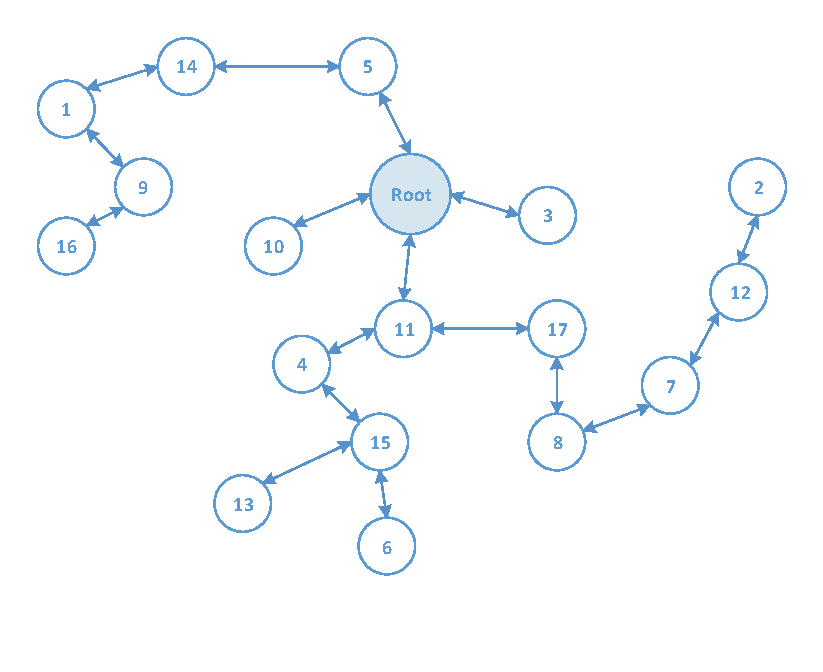
\includegraphics[width=1.0\linewidth]{figures/RPL_DODAG.pdf}
  \caption{A Sample RPL DODAG.}
  \label{fig:rpl_dodag}
\end{figure}

\subsection{Application Layer}

\paragraph{\textbf{\gls{HTTP}}}
\paragraph{}
	\gls{HTTP} is an application level protocol that uses a request-response model and is the foundation of data communication on the \gls{WWW} It is primarily designed to run over \gls{TCP} which is a problem in lossy and constrained environments due to the delivery assurances and congestion control algorithms it employs. Besides, {HTTP} is verbose, text-based, and not suited for compact message exchanges. Moreover, the header size required for a message exchange can leave too few payload space in constrained networks like the IEEE 802.15.4-based networks where the \gls{MTU} size of the protocol is 127 bytes. These protocol specifications would not raise any issues in standard \gls{WWW} communications, but when it comes to constrained environments it is clear that the protocol is not adequate to the necessities of \gls{IoT} devices and networks.

\paragraph{\textbf{\gls{CoAP}}}
\paragraph{}
	\gls{CoAP} \cite{Shelby2014} is a document transfer protocol based on \gls{REST} on top of \gls{HTTP} functionalities. \gls{CoAP} objective is to enable tiny constrained devices to use RESTful interactions, where clients and servers expose and consume web services using \gls{URIs} together with  \gls{HTTP} Get, Post, Put and Delete methods. Unlike \gls{REST}, \gls{CoAP} runs over \gls{UDP} instead of \gls{TCP} which makes it suitable for full IP networking in small micro-controllers. Retries and reordering are implemented at the application stack using a messaging sub-layer that detects duplicated messages and provides reliable communication using different types of messages. Confirmable messages must be acknowledged by the receiver, nonconfirmable follow the fire-and-forget model. Despite being a lightweight protocol, \gls{CoAP} still provides important features:
	
\begin{itemize}
	\item Resource Observation - \gls{CoAP} can extend the \gls{HTTP} request model with the ability to observe a resource therefore monitoring resources of interest using a publish/subscribe mechanism;\\
	\item Resource Discovery - \gls{CoAP} servers provide a list of resources using well-known {URIs} that allow clients to discover what resources are provided and their types;\\
	\item Interoperability - since \gls{CoAP} is based on the \gls{REST} architecture, a simple proxy enables \gls{CoAP} to easily interoperate with \gls{HTTP}.
\end{itemize}

\paragraph{}
A study that compared \gls{CoAP} and \gls{HTTP} using mobile networks concluded that there is no scenario where \gls{CoAP} would consume more resources than \gls{HTTP} \cite{Savolainen2014}.

\paragraph{\textbf{\gls{MQTT}}}
\paragraph{}
	\gls{MQTT} \cite{OASIS2014} is a publish/subscribe messaging protocol designed for lightweight \gls{M2M} communications. It employs a client/server model and consists of three components: the publisher, the subscriber and a broker.
Subscribers register their interest for a specific topic and then get informed by the broker when a publisher generates data regarding that topic. Every message is a discrete chunk of data, opaque to the broker. The broker, on his side, checks authorization of the publishers and subscribers. \gls{MQTT} supports three Application Level \gls{QoS} levels:

\begin{itemize}
	\item At Most Once (Fire and Forget): A message will not be acknowledged by the receiver or stored and redelivered by the sender;\\
	\item At Least Once: It is guaranteed that the message will be delivered to the receiver, but more that one copy can reach the destination due to message resending. The sender stores the message until it gets an acknowledgement from the receiver;\\
	\item Exactly Once: A four-way handshake mechanism is used to guarantee that the message will be received exactly once by the counterpart.
\end{itemize}

\paragraph{}
\gls{MQTT} has support for persistent messages stored on the broker, where the most recent message will be sent to a client that subscribes that topic. Clients can register a custom message to be sent to the broker on disconnect enabling other subscribers to know when a device disconnects. \gls{MQTT} runs on \gls{TCP} which in some cases has drawbacks in performance. A performance evaluation of \gls{MQTT} and \gls{CoAP} \cite{Ma2014} provides comparisons on several protocol facets:

\begin{itemize}
	\item Influence of Packet Loss on Delay: With low values of packet loss, \gls{MQTT} experienced lower delays, but as the packet loss increased \gls{CoAP} performed better. This is due to the greater \gls{TCP} overheads involved in the retransmissions of messages when compared to \gls{UDP};\\
	\item Influence of Packet Loss on Data Transfer: \gls{CoAP} generated less data for each packet loss versus all the \gls{MQTT} \gls{QoS} levels;\\
	\item Overheads for Message Sizes: When packet loss rate is low, \gls{CoAP} generates less overhead than \gls{MQTT} for all message sizes, but as message size grows, the reverse is true. This happens because when the message size is is large, the probability that \gls{UDP} loses the message is higher than \gls{TCP} which causes \gls{CoAP} to retransmit the whole message more often than \gls{MQTT}.
\end{itemize}

\paragraph{}
	In order to address the drawbacks on constrained devices, \gls{MQTT-SN} protocol \cite{Ibm2013} was created. Among the improvements and new features, \gls{MQTT-SN} runs on UDP, adds broker support for indexing topic names, provides a discovery procedure to help clients without a pre-configured server address and supports devices in sleep state. With this approach, an extra gateway is necessary to convert from \gls{MQTT-SN} to \gls{MQTT} so the communications can be understood by the broker.

\subsection{Session Layer}

\paragraph{}
So far, security issues have not been addressed in any of the previous layers. This is because security is an expensive, optional feature. The application layer protocols rely on underneath layers to achieve secure communications, and network layer protocols assume that if security is necessary then it has already been handled in upper layer protocols. In fact, the session layer is where the security mechanisms are implemented and provides an abstraction layer to application layer protocols. These mechanisms work on top of the transport layer and aim to provide authentication, confidentiality and message integrity.

\paragraph{\textbf{\gls{TLS}}}
\paragraph{}
	\gls{TLS} is a well-known security protocol that is used to provide a secure transport layer for \gls{TCP} communications, allowing the upper layer protocols to be left untouched. \gls{TLS} operation consists of two phases: the handshake and then the data encryption. During the handshake, both parties negotiate which algorithms will be used during the session, authenticate themselves, and prepare the shared secret for the data encryption.
	Both \gls{HTTP} and \gls{MQTT} work over \gls{TCP} and use \gls{TLS} as the adopted security protocol.

\paragraph{\textbf{\gls{DTLS}}}
\paragraph{}
	\gls{DTLS} aims to be the equivalent of \gls{TLS} over \gls{UDP} transport layer. \gls{DTLS} works over datagrams that can be lost, duplicated, or received in the wrong order, therefore needing some extra mechanisms (application layer protocols \gls{QoS}) to cope with that. Although both \gls{CoAP} and \gls{MQTT-SN} work over \gls{UDP} and use \gls{DTLS} as the adopted security, some authors argue that \gls{DTLS} is not a suitable option \cite{Alghamdi2013} and defend the need of a new integrated security solution. Some of the presented drawbacks are:

\begin{itemize}
	\item There is no multicast support, which is a key feature in \gls{IoT} (topology discovery and update for example);\\
	\item Handshake phase is prone to exhaustion attacks on the device resources;\\
	\item The loss of a message in-flight requires the retransmission of all the messages in-flight.
\end{itemize}

\paragraph{}
	A final overview of the analysed protocols and security solutions is given in Table \ref{tab:protocols}. And a comparison of the protocol stack is shown in Table \ref{tab:stack}. 

\begin{table}[h]
	\centering
	\begin{center} \caption{\gls{IoT} Application Protocols Comparison} \label{tab:protocols} \end{center}
	\begin{tabular}{c|cccccc}
		\begin{turn}{90}\begin{tabular}{@{}c@{}}Application \\ Protocol\end{tabular}\end{turn} &
		\begin{turn}{90}RESTful\end{turn} &
		\begin{turn}{90}\begin{tabular}{@{}c@{}}Request/ \\ Response\end{tabular}\end{turn} &
		\begin{turn}{90}\begin{tabular}{@{}c@{}}Publish/ \\ Subscribe\end{tabular}\end{turn} &
		\begin{turn}{90}Adjustable \gls{QoS}\end{turn} &
		\begin{turn}{90}Transport\end{turn} &
		\begin{turn}{90}Security\end{turn} \\
		\hline
		\gls{HTTP} & \hspace{0.2cm}\cmark\hspace{0.2cm} & \hspace{0.2cm}\cmark\hspace{0.2cm} &
		 \hspace{0.2cm}\xmark\hspace{0.2cm} & \hspace{0.2cm}\xmark\hspace{0.2cm} & 
		 \hspace{0.2cm}\gls{TCP}\hspace{0.2cm} & \hspace{0.2cm}\gls{TLS}\hspace{0.2cm} \\
		%\hline
		\gls{CoAP} & \cmark & \cmark & \cmark & \cmark & \gls{UDP} & \gls{DTLS} \\
		%\hline
		\gls{MQTT} & \xmark & \xmark & \cmark & \cmark & \gls{TCP} & \gls{TLS}\\
		%\hline
		\gls{MQTT-SN} & \xmark & \xmark & \cmark & \cmark & \gls{UDP} & \gls{DTLS}
	\end{tabular}
\end{table}


\begin{table}[h]
	\centering
	\begin{center} \caption{Protocol Stack Comparison Overview } \label{tab:stack}\end{center}
	\begin{tabular}{c|c|c}
		Layer & Web & IoT \\
		\hline
		Application & \gls{HTTP} & \gls{CoAP} \\
		Session & \gls{TLS} & \gls{DTLS} \\
		Transport & \gls{TCP} & \gls{UDP} \\
		Network & IPv6 & 6LoWPAN \\
		Data-Link/Physical & 802.11 & 802.15.4
	\end{tabular}
\end{table}

\section{Attack Analysis, Detection and Mitigation}
\label{sec:attack_analysis}
\paragraph{}
Exploitation of existing solutions in the forms of malicious attacks can be found at all the studied OSI layers. They can go from a physical intruder replacing some node on a sensor field to the well-known \gls{DoS} at the application layer. However, given the characteristics of the devices and networks used in \gls{IoT} combined with the power consumption focus of this work, a specific kind of attacks performed at the network layer is of special interest and importance: battery depletion attacks, also known as, ``vampire'' attacks.

\paragraph{}
Battery depletion attacks aim at draining the battery, ``life'', of the network devices, working over time to entirely disable a network, hence being called ``vampire'' attacks. These attacks do not focus on flooding the network with many packages, instead they drain the node's life by delaying the packets transmission. Many of the existing attacks are not protocol specific \cite{Vasserman2013}, while others target specific protocols and implementations \cite{Pongle2015}. The following attacks aim at giving an overview of the existing attack possibilities on different routing solutions as well as existing mitigation strategies. Additionally, a range of attacks that target the RPL routing protocol is also analysed. Since RPL is the selected protocol of our energy efficient stack, it is of special importance to consider and assure the mitigation of attacks that would drain the device's batteries by exploiting this light weight protocol's inner workings.   

\subsection{Stateless Protocols}
\label{sec:source_routing}
\paragraph{}
In systems that use this type of routing protocols, the source node specifies the entire route to the destination in the packet header. This means that intermediaries do not make decisions regarding the next hop, they only forward to the next node as specified in the original path therefore reducing the amount of computation performed and used energy. However, the source node must ensure that the route is valid at the time of sending and that the neighbour relations among the devices allow the specified forwarding path. Using this transmission scheme, a malicious device can specify paths through the network that are far from optimal, wasting energy at the intermediate nodes who follow the included malicious source route. The Carousel and Stretch Attacks are examples of these attacks.

\paragraph{\textbf{Carousel Attack}}
\paragraph{}
The objective of this attack is to send a packet along a route composed as a series of loops. This way, a single node may forward the malicious packet several times increasing the total energy consumption by a factor of the number of loops the attacker has introduced on the packet header path. It targets source routing protocols by exploiting the limited verification of the packet headers at the intermediary nodes. Figure \ref{fig:carousel_attack} shows an example where a vampire node created a path composed of circles around the network when it could have exited after the first hop through the D node.
 
\begin{figure}[h]
  \centering
  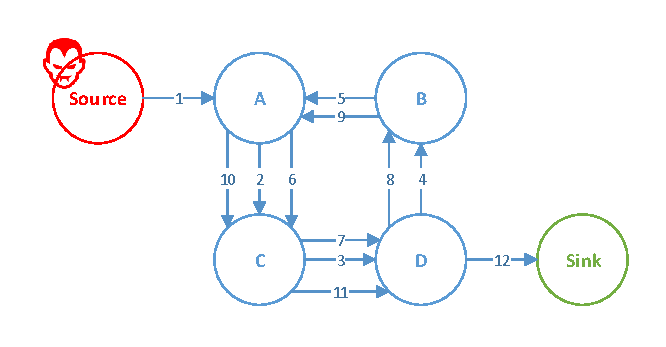
\includegraphics[width=0.9\linewidth]{figures/Carousel_Attack.pdf}
  \caption{Carousel Attack.}
  \label{fig:carousel_attack}
\end{figure}

Existing mitigation strategies rely on checking the source route for loops on intermediary nodes, either selecting an appropriate route for the packet or simply dropping it.

\paragraph{\textbf{Stretch Attack}}
\paragraph{}
The objective of this attack is to create a source route around the network, longer than the one that would be required to transverse the network from the source to the sink. The number of elements in the path would be greater than the optimal path, therefore increasing the total energy consumption by a factor of the number of additional hops. Its success rests on intermediary nodes not checking for better paths. Figure \ref{fig:stretch_attack} shows an example where a vampire node created a path that goes through a greater number of nodes than required to reach the sink.

\begin{figure}[h]
  \centering
  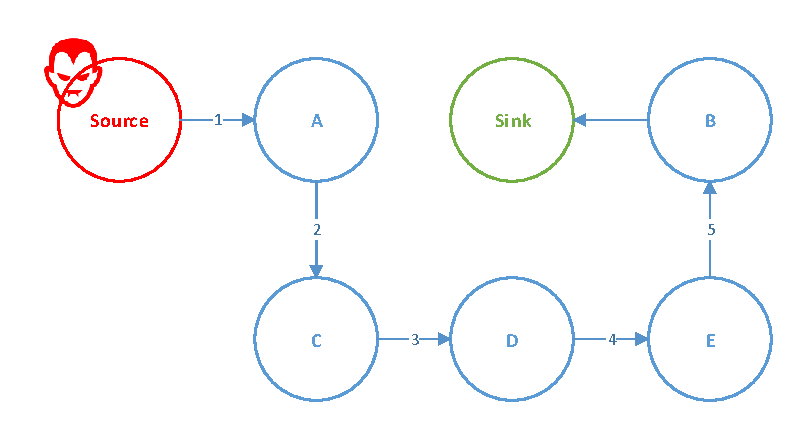
\includegraphics[width=0.8\linewidth]{figures/Stretch_Attack.pdf}
  \caption{Stretch Attack.}
  \label{fig:stretch_attack}
\end{figure}

A limited way of mitigating this attack would be to ensure that path routes have less than the total number of devices on the network. Vasserman and Hoper proposed a property called ``no-backtracking'' that assures the packet is always moving closer to the sink on every hop \cite{Vasserman2013}.
\pagebreak
\subsection{Stateful Protocols}
\label{sec:tables_routing}
\paragraph{}
In systems that use this type of routing protocols, network nodes are aware of the network topology and its state, being able to make local decisions on the node to whom they will forward the packet. The effect of the Vampires on this type of routing is limited since the route is built dynamically from many independent forwarding decisions. However, attackers can still cause damage by forcing packet forwarding through nodes that would not be on the optimal path, for example, by forwarding the packet back to the source. The Directional Antenna and Wormhole Attacks are examples of these attacks.

\paragraph{\textbf{Directional Antenna Attack}}
\paragraph{}
In this attack, the attacker takes the role of an intermediary and not the source of a packet. If the attacker has the resources to use a directional antenna, it can deposit a packet on arbitrary parts of the network while also forwarding the packet locally. This causes nodes that were not on the optimal path to also consume energy by forwarding a packet they would not normally receive, therefore increasing the total energy consumption by a factor of the directions the attacker can position the antenna and the distance between the receiver and the sink. Figure \ref{fig:directional_antenna_attack} shows an example where a ``vampire'' intermediary deposited a node on a distant location of the network, causing the packet to follow two different routes towards its destination

\begin{figure}[h]
  \centering
  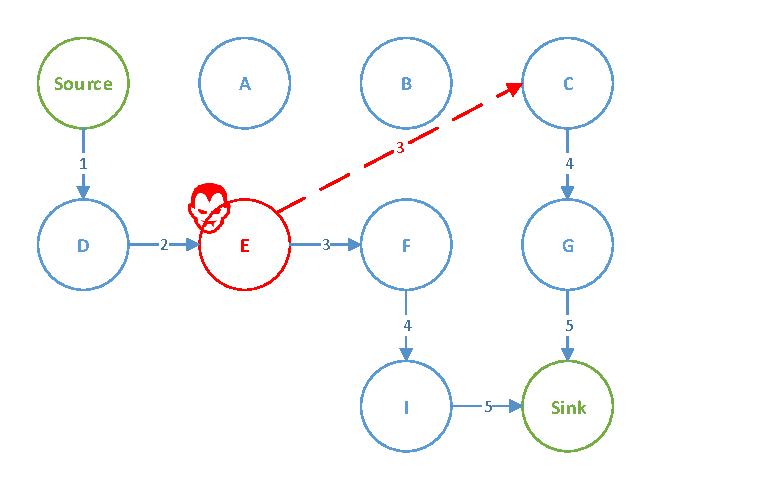
\includegraphics[width=0.8\linewidth]{figures/Directional_Antenna_Attack.pdf}
  \caption{Directional Antenna Attack.}
  \label{fig:directional_antenna_attack}
\end{figure}

A mitigation strategy could be to analyse the route paths of a given packet that reached the sink more than once. The last node identifier to appear duplicated before the path started to diverge would be one who then directed the packet to multiple regions, therefore revealing the attacker.

\paragraph{\textbf{Wormhole Attack}}
\paragraph{}
This attack can be seen as variation of the Directional Antenna Attack but with the collaboration of two or more attackers. Instead of simply forwarding the packets to arbitrary parts of the network, the attacker emulates a link between them and advertises to the network that recently formed connection. This disrupts the topology and has severe impact on routing paths since attackers can indicate that the link cost between them is very low, and therefore influence the forwarding decisions of neighbour nodes. By using these malicious routes, the energy consumption is increased because either this channel does not exist at all (packets are dropped and need to be resent), or the transmission cost between the attackers is greater than the normal message propagation through the network. Figure \ref{fig:wormhole_attack} shows an example where two vampires emulate a connection between them influencing the routing decisions of their neighbours. The hops numbered with prime numbers represent the path taken by a packet after the wormhole is constructed. Although the packet still reached the destination, the cost of the wormhole path is greater than the previous regular path.

\begin{figure}[h]
  \centering
  \includegraphics[width=0.85\linewidth]{figures/Wormhole_attack.pdf}
  \caption{Wormhole Attack.}
  \label{fig:wormhole_attack}
\end{figure} 

Wormhole attacks can be prevented using the Merkle tree authentication \cite{Khan2013}. This tree is organized from the leafs towards the root where every parent knows their children and asks them for authentication based on their ID and public key.
\pagebreak

\subsection{RPL Specific Attacks}
\paragraph{} 


\paragraph{\textbf{Selective Forwarding Attack}}
\paragraph{}
In a selective forwarding attack, a malicious node can launch a \gls{DoS} attack by selectively forwarding packets. Its main goal is to disrupt routing paths but can be used to filter any protocol. Since \gls{RPL} has built in topology repair mechanisms, a full packet filtering would trigger a healing phase and leave the malicious node out of the topology. For sustainability, an attacker could let the RPL control messages pass by and drop the remaining packets. Depending on the routing scheme being used (source routing or stateful tables) the source could first verify path availability or each node could dynamically decide to forward the packet through another path with similar quality. In any case, a good approach would be to report those failures to the underlying RPL system in order to trigger a preventive healing and improve the route quality.

\paragraph{\textbf{Hello Flooding Attack}}
\paragraph{}
The Hello in the name of this attack comes from the initial message a node sends when joining a network. By broadcasting this message with a strong signal power, an attacker can try to introduce himself as neighbour to many nodes of the network, or at least force a large portion of the network to spend energy starting the message exchange for node insertion. A simple solution for this attack would be to test the bi-directionality of the link. If no acknowledgement is received, the path is discarded. Another approach, if geographical locations of the nodes are known, would be to discard every hello message coming from a location beyond the transmission capabilities of ordinary nodes.

\subsection{Protocol Independent Attacks}
\paragraph{}
The last addressed category is not dependant on network topologies or protocol messages. It focuses on attacks that can be performed regardless of the used protocol and whose goal is to obtain information about a network device. With that information an attacker can, for example, try to include himself in the network as a legitimate device or spoof his identity to forward traffic towards him. The Clone and Sybil Attacks are examples of these attacks.

\paragraph{\textbf{Clone ID and Sybil Attack}}
\paragraph{}
As the name suggests, in a clone ID attack, the attacker steals the identity of a legitimate network node by copying the information of that node onto another node. This way the attacker can gain access to the traffic that was destined to the legitimate node, prevent packets to reach their intended destination and can even influence voting schemes. The Sybil attack is similar to the Clone ID, with the difference that the attacker uses several stolen identities on the same physical node. This way, large parts of a network can be taken over without the need to deploy several physical nodes. Figure \ref{fig:clone_attack} shows an example of a clone ID attack where the cloned attacker received the packet that was originally destined to the legitimate node.

\begin{figure}[h]
  \centering
  \includegraphics[width=0.85\linewidth]{figures/Clone_attack.pdf}
  \caption{Clone ID Attack.}
  \label{fig:clone_attack}
\end{figure} 

Proposed mitigation strategies for this type of attacks consist on keeping track of the number of instances of each identity. By using the node neighbours, either a centralized or distributed approach could be used to detect duplicate entries.

\section{Secure Bootstrapping}
\label{sec:secure_bootstrapping}
\paragraph{}
The term bootstrapping is applied to the process in which a new device is connected to an existing network. To achieve a secure bootstrapping, a unique identity and security parameters are associated with the device during this phase. There are several ways to carry out the initial setup, either via a physical interface or wirelessly. In the case of wireless bootstrapping, attention must be given to eavesdropping so that the secure credentials cannot be intercepted.\\
Since many of the studied attacks are to be performed by a malicious intruder capable of interacting with the network, if we could assure a secure bootstrapping, meaning that the new node would be authenticated before becoming an active member of the network, a large portion of those attacks could no longer be performed. The following bootstrapping techniques were summarized in \cite{Fischer2012} and aim at providing secure bootstrapping for \gls{IoT} devices.

\subsection{Token-Based}
\paragraph{}
In token-based distribution, device specific security credentials are generated and written to a token. That token can range from memory sticks or flash cards to \gls{RFID} tags or smartcards. Is has the advantage that this initial credential generation can be performed on a physically controlled environment and only later, on the commissioning phase, is the token plugged into the device. After the successful insertion of the security credentials, the token can be removed and collected back into the secure environment. This process can be considered of high security since the credentials are generated on a closed environment and are transmitted through a physical link. To further increase the security level, a password could be used to encrypt the credentials, however, that would require the device to have some kind of interface that would allow to input the password. In the case of a large number of devices, this approach would be unsuitable due to the management effort of manually deploying the tokens to the devices \cite{Fischer2012}.

\subsection{Identifier-Based Access Control List}
\paragraph{}
With an identifier based \gls{ACL}, new devices are allowed or denied access to the network based on their unique ID. A commonly used identifier is the MAC address. This has some major drawbacks in security since, firstly, it provides no assurances on the first time the device connects to the network. An attacker can easily intercept the first messages and get access to the device information. And secondly, after the bootstrapping phase, MAC addresses can be spoofed by an attacker, allowing him access to the network by bypassing the \gls{ACL} with the identifier of a legitimate node.

\subsection{One-Time-Passwords}
\paragraph{}
The use of one-time-passwords enhances the manual input of credentials on the device to be bootstrapped. The person responsible for the deployment of the new node should receive through a secure channel an one-time-password, that would then be used to authenticate the node, by authenticating its locally generated key material. This material can be either a certificate request to a \gls{CA} or a locally generated public/private key pair. The achieved security level is proportional to the security of the channel used to obtain the one time password, but assuming that channel is secure, so is this method. The drawback is that it forces devices to possess some kind of interface to insert the one time password.

\subsection{Manufacturer Installed Credentials}
\paragraph{}
So far, excluding the identifier based access control list, the intent of the studied techniques is to supply to the new device the security credentials needed to obtain access to the network, or at least provide an authentication method that allows fetching those credentials. In manufacturer installed credentials, those security credentials are deployed during the manufacturing process of the device vendor. Those credentials are typically a public/private key pair certificate bound to the identifier of the device. This certificate can be integrated into the initial loading of the firmware or stored in a separate integrated circuit designed for credential storing. In the second case, this method's security can be considered very high since those integrated circuits assure that the private key cannot be read from memory. This way, the new device comes shipped with the necessary security credentials not only for the bootstrapping phase but also for the normal operation phase since it does not need to fetch any additional credentials. The effort is on the root or management station that needs to import the vendor \gls{CA} certificates to assure the new device credentials are trustworthy. Also the production costs increase, implying an increased device cost.

\subsection{Recently Proposed Solutions}
\paragraph{}
Secure bootstrapping and network admission solutions have already been proposed in past literature. However, the development and optimization of application layer protocols as well as network layer routing schemes allows for new approaches and solutions that can now fit the nature of \gls{IoT} devices.
Bergman et al. \cite{Bergmann2012} proposed a three-phase secure bootstrapping technique for nodes in a \gls{CoAP} network. Firstly the joining node broadcasts a request for a \gls{CSDS}. This server, once contacted by a new node takes the responsibility of key distribution. Then the system goes under a vulnerable phase where the secret is transmitted from the \gls{CSDS} onto the new device. The author's proposes a short audible or visual feedback to the human installer when the secret is received and assumes that potential eavesdroppers can not intercept this transmission. Finally, this secret is used to setup the \gls{DTLS} connection. This approach has major security drawbacks. On the secret transmission phase, so the authors propose limiting the radio power to a low level and disable data forwarding beyond the local network segment, but these techniques cannot assure that an attacker won't be able to intercept the transmission.\\
Oliveira et al. \cite{Oliveira2013} proposed an admission control solution for 6LoWPAN networks based on administrative approval. Each joining node would broadcast its presence to the network, and that broadcast would be received by the administrator in the management server. Then, the administrator would grant access to that new device based on its address, and that information would be transmitted to all the devices in the network. After this phase, the device would be allowed communication as a regular member of the network by its neighbours. This approach has the advantage of requiring no previous setup on the device before operation but is vulnerable to the attacks previously mentioned in identifier based \gls{ACL}. The authors state that work still needs to be performed in order to validate the sensor identity and leave as possibility the pre-instalment of keys on the device. 
%TEX root = ../dissertation.tex

\chapter{Proposed Solution}
\label{chapter:proposed_solution}

Before attempting to develop a protocol, or solution, that meets our goals and properly addresses the problems and attacks described in the previous chapters, it is important to define the scope of our work. A common appropriate way to do so is by presenting both a scenario and architecture of the solution. The Internet of Things is currently a hot trend and this work could potentially apply and benefit a wide spectrum of applications, ranging from home environments to large enterprise networks. However, these are domains that have different requirements. A home application should be easy to setup and not require complex configurations to the user. An enterprise solution can benefit from additional administrative configurations as long as the deployment of the devices can be done quickly and easily due to their potential large number. Our work will position itself in the middle of these two domains. We are looking at a complexity and number of devices greater than a home environment but it is not our focus to provide solutions for enterprise networks and their deployment restrictions. It is our belief that a Smart University Campus is an adequate scenario and can effectively demonstrate the needs targeted by our work. In the following sections we will apply the information gathered in the related work sections to formally define what we are trying to achieve, what are the difficulties in achieving those goals and how can we overcome them. Then, a model of a campus with the proposed energy-efficient network architecture will be presented and their component roles explained. 

\section{Planning}

\subsection{Objectives and Requirements}
\paragraph{}
One of the major concerns regarding \gls{IoT} application is the communication model. For our work, we pose as requirement that the system is power-aware and uses the minimum energy possible. Additionally, the following set of objectives is desirable to build trust and allow secure communications to take place.

\begin{itemize}
	\item Confidentiality: Without confidential message transmission, packets would flow in the network in plain text. Attackers could sniff the packets in order to obtain information, and depending on the application, this could be a security breach. Even if there is no critical data being sent, privacy is still compromised.\\
	\item Integrity: Assuring message integrity means that the message was not modified between the source and its destination. Without integrity we could not rely on the received data since it could have been, intentionally or not, modified on the fly, and be providing the system wrong information.\\
	\item Authentication: The studied type of networks relies on hop-to-hop communication, meaning several nodes will take place in forwarding a packet. If they are not authenticated they could perform a wide range of attacks and disrupt the network.
\end{itemize}

\subsection{System Architecture and Message Flow}
\paragraph{}

As stated in the beginning of the chapter, we will use a Smart Campus scenario. Being aware of the technological improvements on sensor networks and building management technologies, the \gls{IST} administration decided to improve the monitoring the overall conditions of the buildings and inside environments in order to better preserve its assets. To cope with the new requirements, we propose a solution for the monitoring of the campus sections by deploying a wireless sensor network on each building, connected to a central management station operated by the available staff. The scenario will be based on the \gls{IST} campus model. An overview of the system and its components over the \gls{IST} blueprints can be found in Figure \ref{fig:global_architecture}. Regarding each individual component:

\begin{itemize}
	\item Numeric Nodes: Represent the network sensor nodes, the most constrained element of the network. They cooperate to build the topology and route messages hop-by-hop until the root is reached. These are fully equipped with the energy efficient protocol stack defined in Section 4.1\\
	\item Alphabetical Nodes: Represent the root node of each section network topology. They are equipped with the same stack of the numbered nodes but are more powerful, preferentially not battery powered and act as the bridge between the constrained 6LoWPAN environment and the central management station. These nodes must be more powerful than the numeric ones so that they can process all the requests between a group of sensors and the management station. Also, although the numeric nodes use low-power wireless radios, the alphabetical nodes must be capable of interfacing with more power hungry radios and protocols therefore requiring more resources. This differentiation allows numeric nodes (the large portion of the network devices) to keep their very constrained nature, consuming less energy, an still be able to communicate with external devices.\\
	\item Management Station: A black box model of the core components of the system. Each building reports to the central station and the staff monitors the status through it. A white box model will be shown in the following sections.\\
	\item Client: The system's clients can be any user with access credentials, but mostly the staff members. They can access the management station either from within the local network or from outside through the Internet.\\
\end{itemize}
 
\begin{figure}[h]
  \centering
  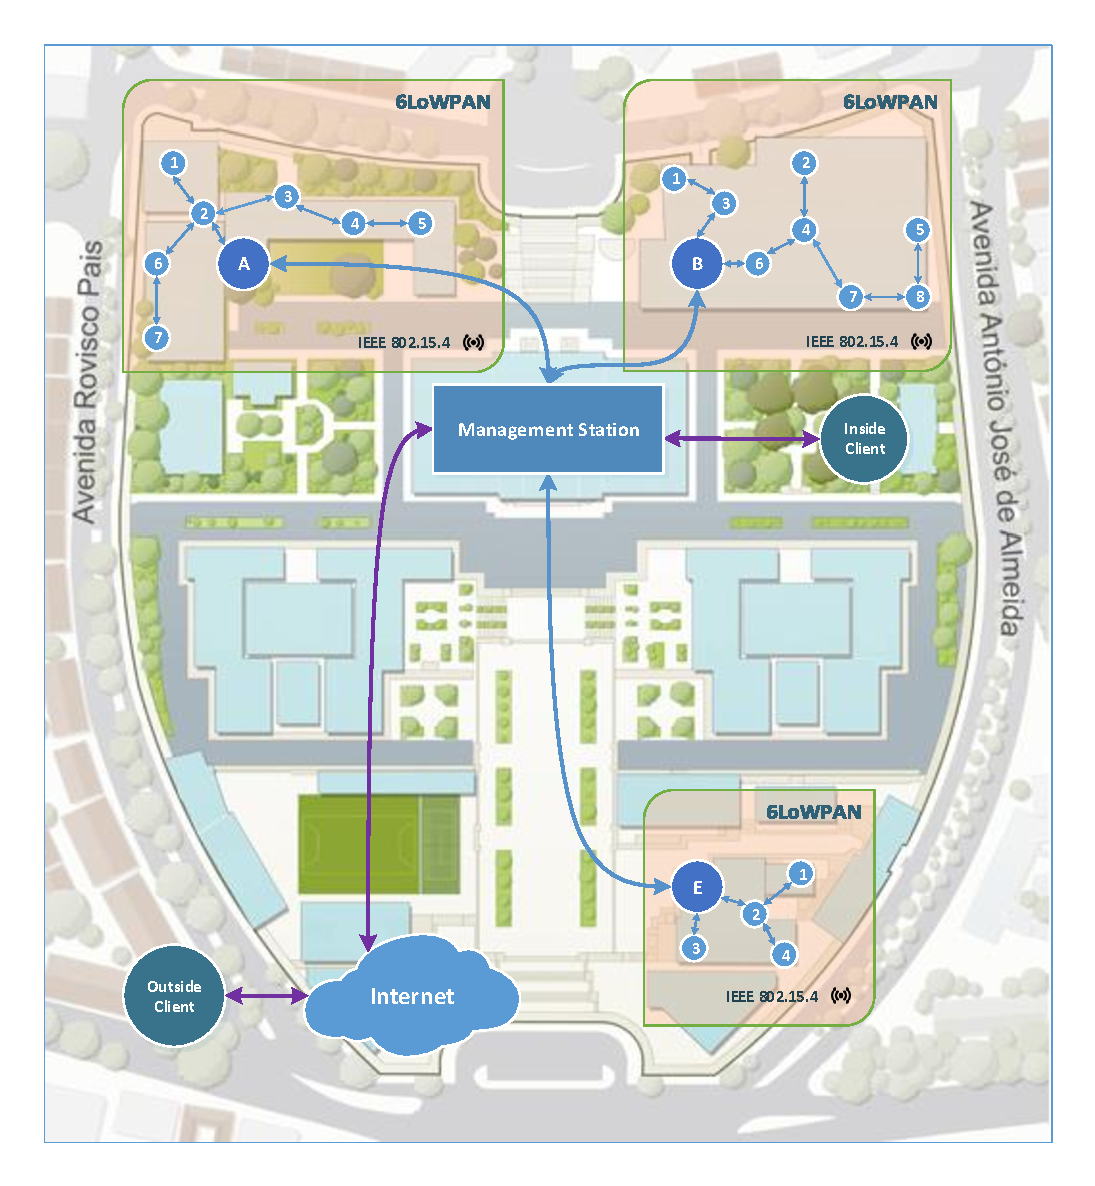
\includegraphics[width=0.9\linewidth]{figures/Global_Architecture.pdf}
  \caption{Global System Architecture}
  \label{fig:global_architecture}
\end{figure}

\paragraph{\textbf{Central Management Station}}
\paragraph{}

The central management station is divided in five main components. A white box schematic of the core components and interactions can be found in Figure \ref{fig:core_components}. Regarding each individual component:

\begin{itemize}
	\item Key Store: This component is responsible for storing the shared network key for the RPL protocol and a mapping between each network device and its key pair. This information is facilitated to the Client Observer for creating a secure connection to each sensor node;\\
	\item Bootstrapper: The bootstrapper acts as the interface between the management station and the network devices. It generates the device key pair and writes it together with the shared network key and the Client Observer public key into the new device;\\
	\item CoAP Client Observer:  The one and only client in the network. Instead of the user directly requesting the sensor readings, the client will observe each resource and be notified of the new value. Each time it receives an update, it stores the information on the Data Server for the clients to use;\\
	\item Data Server: A database with mappings of each node to the most up to date value reported. It's updated by the client observer and used on demand by the clients;\\
	\item Proxy: Responsible for bridging requests coming from the Internet to the Data Server. Responsible for authenticating the external clients and providing access to the Data Server information.\\
\end{itemize}

Although each user could access the system through a \gls{CoAP} terminal and request the most up-to-date readings from the sensor nodes, this approach would cause many overheads in the system. Firstly, and since many clients can connect from different locations, many requests would be performed to the sensor nodes for the same information. Additionally each sensor node would need to be pre-installed with the public keys of all the different user terminals. This would mean additional memory usage in the physical devices, and more requests to the already constrained battery operated network. With the single client approach acting as an observer, only one message needs to go through the network for each new reading.

\begin{figure}[h]
  \centering
  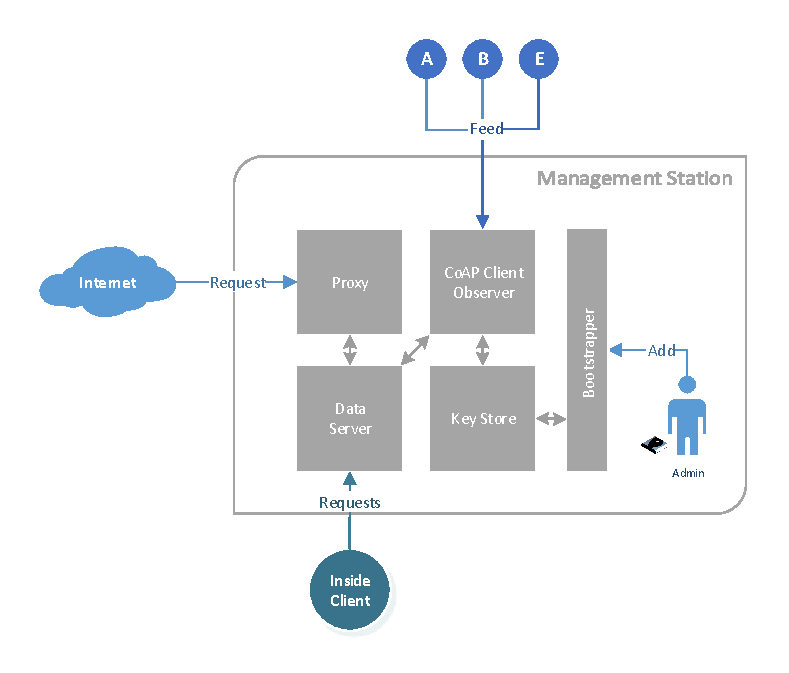
\includegraphics[width=0.92\linewidth]{figures/White_Box_Model.pdf}
  \caption{Central Management Station}
  \label{fig:core_components}
\end{figure}

\paragraph{\textbf{Credentials Configuration}}
\paragraph{}

In order to achieve secure communications, the new node must connect to the RPL network in a secure way, that is by using a pre-shared group key. After that network setup, it will also need to make a DTLS handshake with the client observer, for that needing a key pair and the public key of the client observer. That information is written into the device during the configuration phase, done by the staff members. Figure \ref{fig:sequence_bootstrapping} shows a sequence diagram of the initial configuration phase. This process will be fully automated without requiring the staff administrator any knowledge of the inner workings of the network and authentication procedures.

\begin{figure}[h]
  \centering
  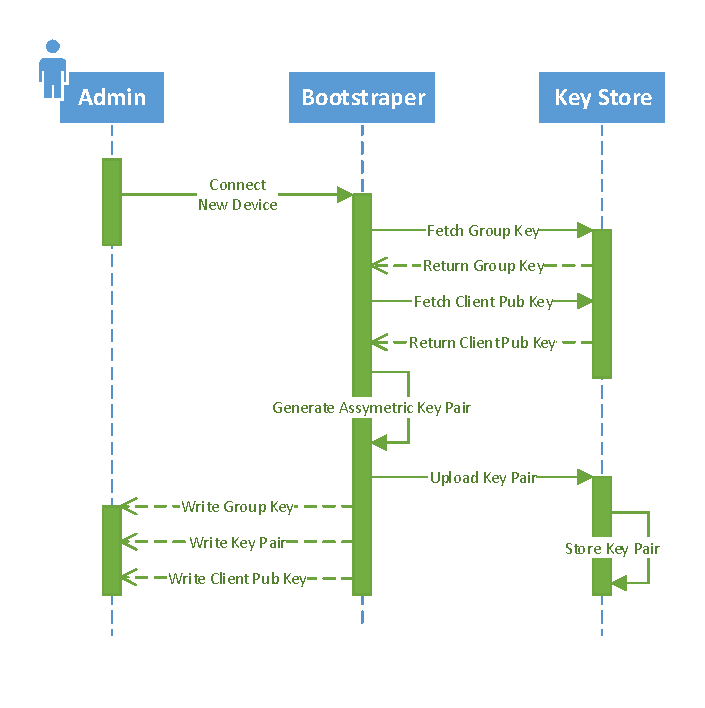
\includegraphics[width=0.8\linewidth]{figures/Sequence_Bootstrapping.pdf}
  \caption{New Device Initial Configuration}
  \label{fig:sequence_bootstrapping}
\end{figure}

As shown in the sequence diagram, the process is initiated by a staff member by connecting a new device to the bootstrapper. The bootstrapper automatically requests the network group key from the key store and the Client Observer public key. Then a new key pair is generated and stored in the key store for that device. Finally the bootstrapper writes the group key, the key pair and the Client Observer public key into the device.
\pagebreak
\paragraph{\textbf{Network Layer Bootstrapping}}
\paragraph{}

After the credentials configuration phase, the new device is fully equipped with the security credentials required for joining the RPL network. Figure \ref{fig:sequence_network_admission} shows a sequence diagram of process started by the new node to join the network topology. The vocabulary used to represent the message exchange was previously presented in Section \ref{sec:network_layer}. All the message exchange is done with the secure versions of the RPL control messages, meaning the data is cyphered with the shared group key.

\begin{figure}[h]
  \centering
  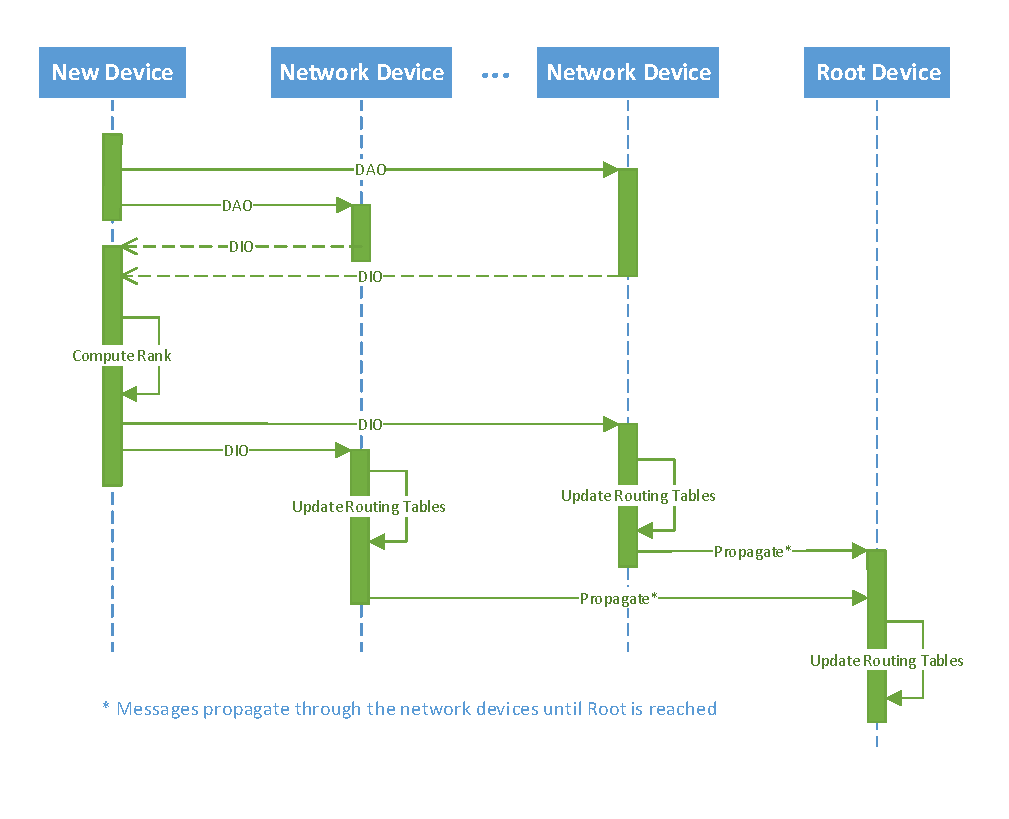
\includegraphics[width=0.95\linewidth]{figures/Sequence_Network_Admission.pdf}
  \caption{Network Layer Bootstrapping}
  \label{fig:sequence_network_admission}
\end{figure}

As shown in the sequence diagram, the process is initiated by the joining device by broadcasting \gls{DAO} messages to any available neighbour devices in range. The receiving nodes will reply to the new device with a \gls{DIO} message that provides graph routing information. With this information the new device is able to compute its rank (the distance towards the root) and define its parents based on that metric. After that process is complete, the new device tells his neighbours about its position in the graph using a \gls{DIO} message and the receiving nodes update their routing tables so that downwards traffic can now reach the new node. This information is further propagated up the network topology until the root is reached.

\paragraph{\textbf{Application Layer Bootstrapping}}
\paragraph{}

Although the device is now bootstrapped at the network layer, it still needs to discover and be discovered at the application layer. This means contacting the Client Observer, securing the channel through \gls{DTLS} and then send new readings as they occur. Figure \ref{fig:sequence_application_admission} shows a sequence diagram of process started by the new node to join the \gls{CoAP} network.

\begin{figure}[h]
  \centering
  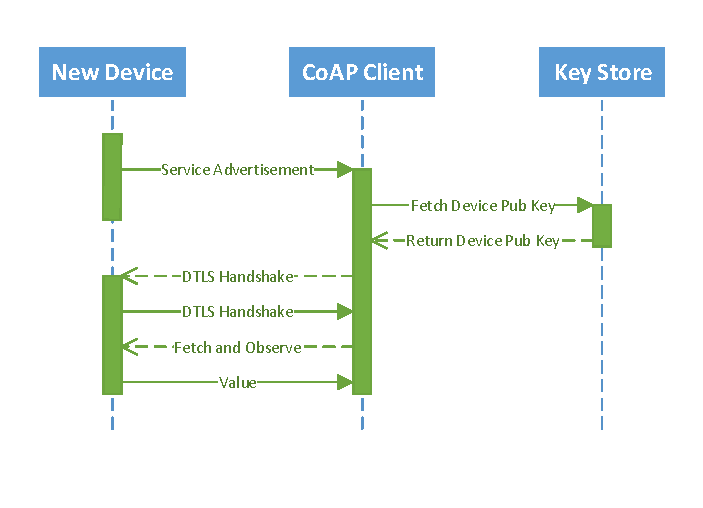
\includegraphics[width=0.8\linewidth]{figures/Sequence_Application_Admission.pdf}
  \caption{Application Layer Bootstrapping}
  \label{fig:sequence_application_admission}
\end{figure}

As shown in the sequence diagram the process is started by the new device that advertises its services to the network. That message is eventually received by the Client Observer who uses the new device public key, stored in the key store to start a \gls{DTLS} secured channel. After the handshake is completed, the Client Observer requests the latest readings to the sensor and sets the observe option meaning each time there is a change in the sensor reading the client will be notified.

\section{Implementation}

\subsection{Network Devices}

\paragraph{\textbf{Operative System}}
\paragraph{}
The greatest planning challenge involved in deploying the network devices was connecting all the proposed protocol at the different layers together. To achieve this, several operative systems for constrained devices were examined attempting to understand how they worked and what features did they offer. The operative systems under comparison were Contiki-OS\footnote{http://www.contiki-os.org/}, TinyOS\footnote{http://tinyos.stanford.edu/tinyos-wiki/index.php/FAQ} and RIOT-OS\footnote{https://riot-os.org/}\\
After examination of the source code repositories, wiki pages and community mailing lists, we could understand that RIOT is the newest and more ambitious, attempting real time processing and claiming to support "all relevant open standards" for the \gls{IoT} but still in a starting phase and lacking complete implementations of some protocols and still working on developing drivers for the most recent hardware platforms. Regarding TinyOS, it follows a less ambitious approach, presenting itself as a work scheduler with a collection of drivers for micro-controllers. Unfortunately, it appears to have stopped in time, with the latest release being dated August 2012 and not supporting the latest hardware boards. Contiki-OS on the other hand claims to be a "powerful box for building complex wireless systems". According to the documentation it supports all the protocols required and has recently published drivers for the most recent hardware platforms. It also ships with a network simulator, allegedly allowing to construct a virtual network that accurately mimics a real deployment on hardware. The combination of these factors led to the choosing of Contiki-OS as the operative systems for our network nodes. Figure \ref{fig:stack_operative_system} acts as a reminder of the attempted protocol stack, alongside with the selected operative system.\\

\begin{figure}[h]
  \centering
  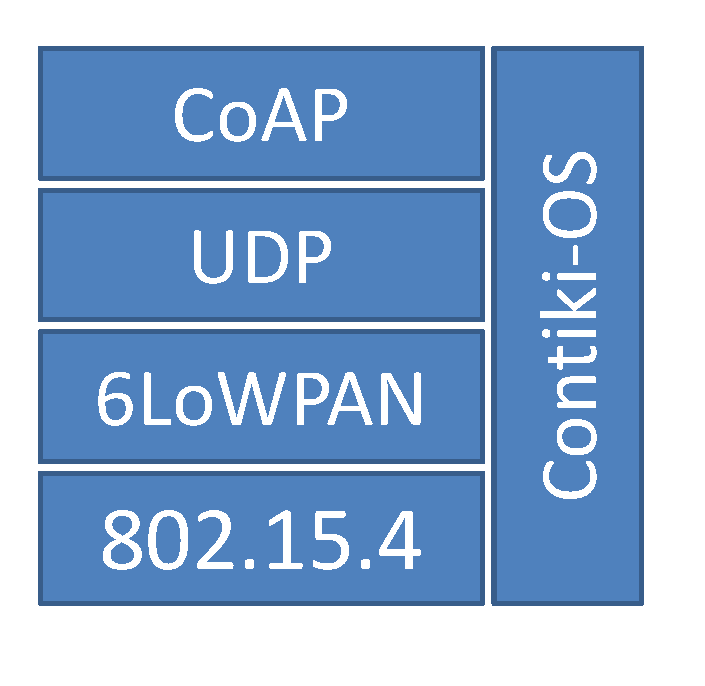
\includegraphics[width=0.3\linewidth]{figures/Stack.pdf}
  \caption{Protocol Stack and Operative System}
  \label{fig:stack_operative_system}
\end{figure}

With respect to the Contiki-OS internal structure, the operative system has been divided by category folders at the root level, similar to what can be found on a regular Linux distribution. The most relevant and that required greatest attention and understanding for this work are presented as follows:

\begin{itemize}
	\item \textbf{apps} - in this folder lies the code for applications, like telnet, ping, mqtt and our desired application layer protocol - \gls{CoAP};
	\item \textbf{core/net} - in this folder, the code responsible for networking is found, particularly our desired network layer protocol - RPL. IPv6 and link layer security are also implemented;
	\item \textbf{platform} - in this folder we can find the drivers for the supported platforms;
	\item \textbf{examples} - in this folder, simple working examples of many apps can be found, including \gls{CoAP};
	\item \textbf{tools} - in this folder we find non-essential apps that can help if we want for example to measure resource consumptions on real hardware.
\end{itemize}

\paragraph{\textbf{Application and Session Layer}}
\paragraph{}

Although applications should now come out-of-the-box with the selected operative system, \gls{CoAP} configuration and the creation of the application endpoints that will be accessed by the network clients on the management station needs to be done by the developer. These endpoints also increase in complexity when accessing specific hardware like humidity and temperature sensors, or when we want observable resources, where when a change occurs an event is triggered that will notify all the resource observers. In our work, we wanted to imprint on the devices an unique identifier, therefore needing to implement a simple text resource, and also make use of the hardware capabilities to create a live network, resorting to the sensors included on hardware. This implied the creation of endpoints capable of interacting with hardware devices and configuring those endpoints to be observable by the \gls{CoAP} clients. The following snippets present an overview of what is required for creating observable \gls{CoAP} endpoints.\\
Firstly, it is necessary to declare a new resource. Since we will be creating a temperature resource, and temperatures change without human intervention, it needs to be declared as n periodic resource in order to trigger periodic temperature reading events. Besides the title, it needs a handler function that runs when the endpoint is reached by a client, and a periodic handler function that runs when a specified amount of time is reached.

\begin{lstlisting}
PERIODIC_RESOURCE(res_temperature,
         "title=\"Temperature\";rt=\"Temperature\";obs",
         res_get_handler,
         NULL,
         NULL,
         NULL,
         CLOCK_SECOND,
         res_periodic_handler);
\end{lstlisting}

The handler function is responsible for returning the most up-to-date value on the resource being requested. To do this, if first reads the latest value directly from hardware, and then construct the appropriate response using the fetched value.

\begin{lstlisting}
static void
res_get_handler(void *request, void *response, uint8_t *buffer, uint16_t preferred_size, int32_t *offset)
{

  int temperature = temperature_sensor.value(0);

  REST.set_header_content_type(response, REST.type.TEXT_PLAIN);
  snprintf((char *)buffer, REST_MAX_CHUNK_SIZE, "%d", temperature);

  REST.set_response_payload(response, (uint8_t *)buffer, strlen((char *)buffer));
  REST.set_header_max_age(response, MAX_AGE);
\end{lstlisting}

The periodic handler function is responsible for monitoring the resource and if it detects changes to the value, within a configured range, it sends messages to all the registered resource observers with the most up-to-date value.

\begin{lstlisting}
static void
res_periodic_handler()
{
  int temperature = cc2538_temp_sensor.value(1);

  ++interval_counter;

  if((abs(temperature - temperature_old) >= CHANGE && interval_counter >= INTERVAL_MIN) || 
     interval_counter >= INTERVAL_MAX) {
     interval_counter = 0;
     temperature_old = temperature;
    /* Notify the registered observers which will trigger the res_get_handler to create the response. */
    REST.notify_subscribers(&res_temp);
  }
}
\end{lstlisting}

Finally, the created resources need to be activated in the \gls{CoAP} main process so that they will become visible to clients requesting the resources that server is making available. Additionally, it is necessary to activate hardware specific components that are being used in those endpoints, in this case the temperature sensor. After these declarations are run, Contiki-OS will provide the necessary data structures and pointers to interact with the resource and make them available for the previously seen handlers. This is one of the big advantages of working with a operative system that supports both the application layer protocols and target hardware.

\begin{lstlisting}
PROCESS_THREAD(coap_server, ev, data) s
{
  PROCESS_BEGIN();

  PROCESS_PAUSE();

  /* Initialize the REST engine. */
  rest_init_engine();

  /* Initialize project specific endpoints */
  rest_activate_resource(&res_id, "info/id");
  rest_activate_resource(&res_event, "sensors/button");
  rest_activate_resource(&res_temp, "sensors/temperature");

  /* Initialize board specific drivers */
  SENSORS_ACTIVATE(cc2538_temp_sensor);
  PROCESS_END();
}
\end{lstlisting}

After having a working \gls{CoAP} server, the focus moved to securing the communications at the session layer, as planned, using \gls{DTLS}. Unfortunately this goal was never achieved due to the lack of compatibility between the available \gls{DTLS} implementations, the used operative system and the selected hardware board. Although many attempts have been made, using implementations from different sources \footnote{https://github.com/cetic/6lbr/wiki/Example-:-Dtls-Coap-Server} a running setup was never achieved. As an extreme option, moving towards another operative system (TinyOS) was attempted, and even using the "supported" \gls{DTLS} implementation from that system, it was not possible to achieve a running example since it had only been tested on old hardware and was not working with the most up-to-date boards available. After submiting bug reports and trying to get help from the community with no practical results the usage of \gls{DTLS} was abandoned since the time required to do adapt an existing implementation to our working setup would take more time than the available to complete this project.

\paragraph{\textbf{Network Layer}}
\paragraph{}

Regarding the implementations at the network layer, the desired routing protocol, \gls{RPL}, should work out-of-the-box with the selected operative system and indeed it did. However some small adjustments and configurations needed to be made so that the total amount of allocated space for routing tables could fit the target hardware. These tweaks were made in the \gls{RPL} configurations file and resorted to limiting the amount of neighbours and max-routes per device. A maximum of twenty routes and twenty neighbours was chosen since it was far superior to the required for this project and believed to be a reasonable number for the smart campus scenario under consideration.

\begin{lstlisting}

#ifndef NBR_TABLE_CONF_MAX_NEIGHBORS
#define NBR_TABLE_CONF_MAX_NEIGHBORS                20
#endif
#ifndef UIP_CONF_MAX_ROUTES
#define UIP_CONF_MAX_ROUTES                 20
#endif

\end{lstlisting}

Once the network layer was working and it was possible to see the topology being formed, the focus moved to enable the secure variation of the \gls{RPL} messages that would authenticate them and prevent the vampires from joining the network. Unfortunately, when the developers of Contiki-OS implemented the \gls{RPL} protocol for their operative system, left out the secure variations of the protocol control messages as fixed in the \gls{RPL} RFC document \footnote{https://tools.ietf.org/html/rfc6550}. Since this was a mandatory feature for the whole purpose of this work, alternatives needed to be found, and after contacting the developers behind the \gls{RPL} implementation for Contiki-OS, i was advised to use \gls{LLSec} as an alternative.\\
\gls{LLSec} works by cyphering packets at the link-layer, right before leaving the host. Those packets are then deciphered upon reaching the next device. This process repeats itself until the destination is reached. In the case of Ad-Hoc networks like this one, the proposed alternative was achievable, and an implementation of \gls{LLSec} was already present in Contiki-OS. To make use of \gls{LLSec}, a network-wide key needed to be flashed onto the hardware that would then be used for the packet cyphering. More in depth, the security credential provided to the joining nodes is a 128bit key, used for the \gls{AES} \cite{Fips2001} in \gls{CCM} star mode \cite{Corp2005}. This allows packets to have their payload encrypted and the message authenticated with a \gls{MIC} also computed from the AES-128 key. This assures that all the packets flowing through the network, even the joining node first communications, are confidential and authentic therefore fulfilling the requirements for this layer. Further explanations of this bootstrapping phase will be given in the Central Management Station section \ref{backend_services}.

\subsection{Border Router}

The border router is the network component that creates the bridge between the \gls{6LoWPAN} network and the outside world. This means that the device will need to have two interfaces, one with the 802.15.4 radio and another one to connect to the outside networks. The border router can and should be permanently connected to a power source, meaning that its power consumption is not an issue. Also, it should be more powerful than the remaining network devices because it will be in charge of taking care of all the packets going inside and outside the \gls{6LoWPAN} network. After analysing the available border router solutions, the implementation from \gls{CETIC} \footnote{https://github.com/cetic/6lbr/} was selected because it provides a deployment-ready solution that runs out-of-the-box on Linux hosts, supports various network topologies, is in active development, has releases from this year (2016) and an active community. Considering this option, the well known Raspberry Pi \footnote{https://www.raspberrypi.org/} board was selected to be the host of the \gls{CETIC} solution due to its more capable hardware, widespread use and full support from the border router distribution. Since the Raspberry platform does not possess an 802.15.4 radio interface, one of the network hardware boards was used as the radio for the border router, a solution that is also fully supported by the \gls{CETIC} distribution. Figure \ref{fig:border_router_setup} shows the border router setup used for this work and its connections to the central management station

\begin{figure}[h]
  \centering
  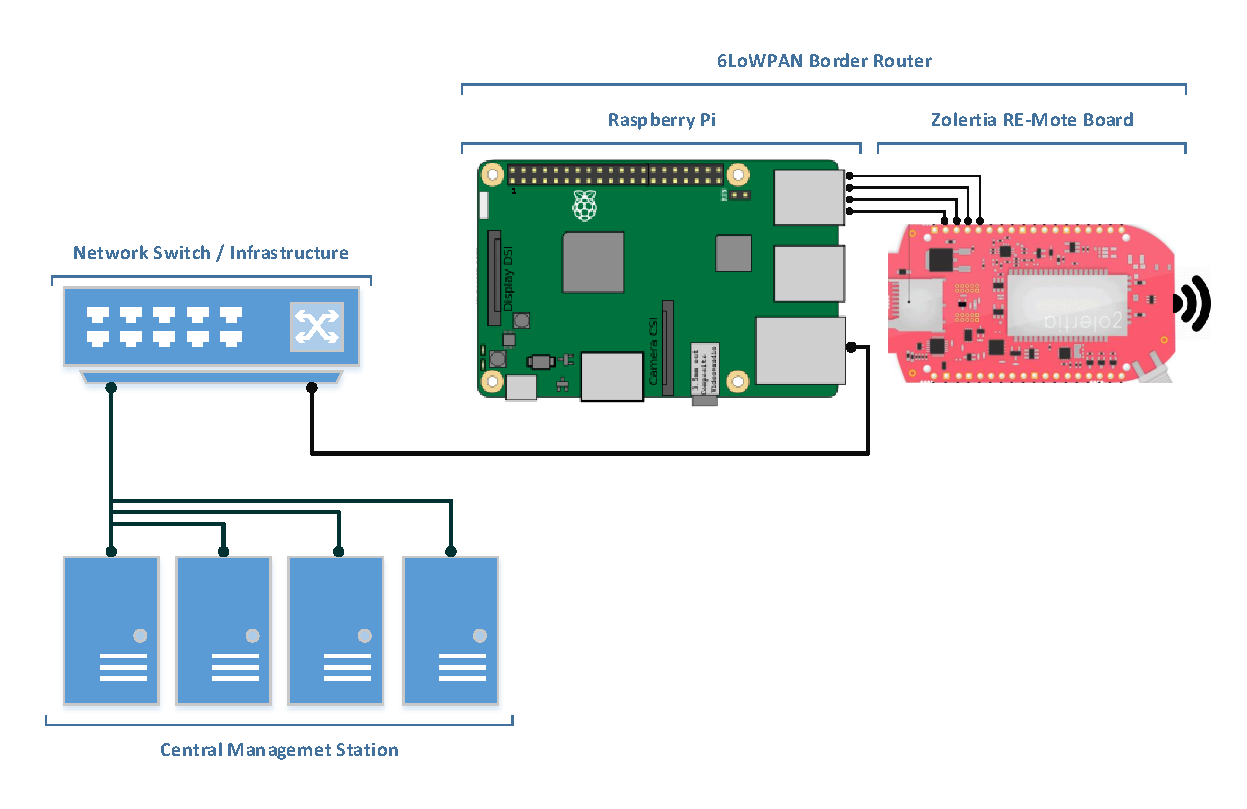
\includegraphics[width=1.0\linewidth]{figures/Border_Router.pdf}
  \caption{Border Router Setup}
  \label{fig:border_router_setup}
\end{figure}

For the border router to become active, firstly a Linux distribution needs to be installed on the device. In this work, the Raspbian \footnote{https://www.raspberrypi.org/downloads/raspbian/} distro was used due to its widespread use and support. Then, \gls{CETIC}'s border router implementation needs to be installed as a service running on the Linux host. This is done by firstly installing the required dependencies, followed by compiling the sources and then starting the service.

\begin{lstlisting}

sudo apt-get install libncurses5-dev
sudo apt-get install bridge-utils

make all
make plugins
make tools

sudo make install
sudo systemctl daemon-reload
sudo service 6lbr start

\end{lstlisting}

Now all that is left to do is flash the hardware board providing 802.15.4 communications. Within the sources for the border router we can find the executables for flashing this board with the slip radio firmware. This can be done with the following command:

\begin{lstlisting}

make TARGET=remote slip-radio.upload

\end{lstlisting}

In the case of plain-text communications, no additional steps were required for operation, and the border router solution should be working as the topology root and immediately adding any servers within reach to the network. However, since our solutions makes use of \gls{LLSec} it is required that the border router learns the network key. The border router will always be the destination of all packets going outside the \gls{6LoWPAN} network and the final deciphering point for the message packets. This can be done on the border router administration page as presented in Figure \ref{fig:administration_page}

\begin{figure}[h]
  \centering
  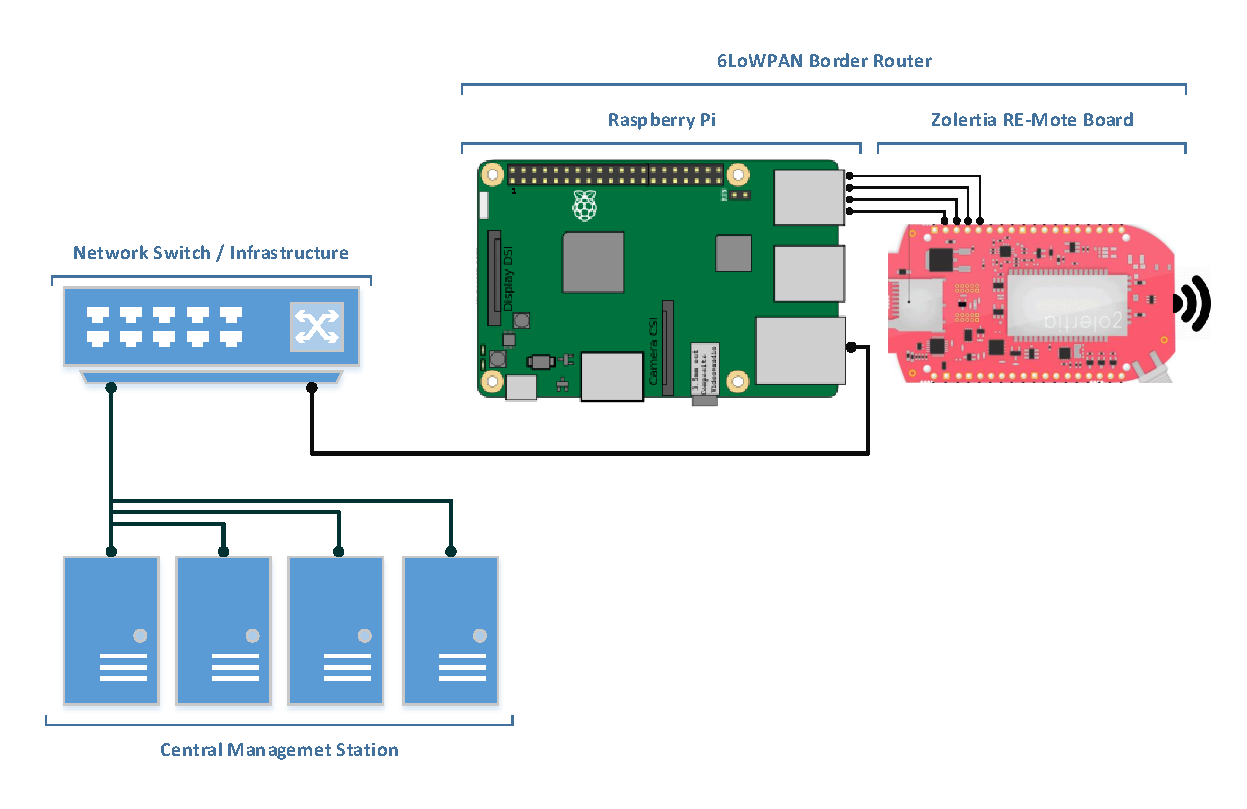
\includegraphics[width=0.8\linewidth]{figures/Border_Router.pdf}
  \caption{Border Router Administration Page}
  \label{fig:administration_page}
\end{figure}



\subsection{Central Management Station}
\label{backend_services}

wepinwe
wepdinwepid
\section{Execution}

weojndweod
wepidnweoid

\section{Limitations and Future Work}
\paragraph{}
The use of secure RPL messages with the pre-shared group key together with the raw public/private key pairs assures that a new device is properly authenticated when joining the network as well as confidentiality and integrity of the propagated packets. However, public key cryptography is based on computationally intensive mathematical functions that are not very efficient on constrained devices. In fact, asymmetric encryption techniques are almost 1000 times slower than symmetric techniques because they require more computational processing power \cite{Kumar2011}. In the event that our work reveals the impossibility to use public key cryptography on the most constrained sensing nodes, symmetric cryptography is hereby posed as an alternative.\\
Also, as discussed in Section \ref{sec:attack_analysis}, an attacker could try to introduce himself in the network by stealing the keys from a deployed device. The solutions for that attack can be either software based, assuring that secure memory areas cannot be copied to external locations. Or hardware based, certain integrated circuits assure the stored information cannot be read from them \cite{Lesjak2014}. This attack will not be mitigated in our system as we believe the mitigation strategies are outside the scope of this project and more related to other engineering fields of research.\\
%!TEX root = ../dissertation.tex

\chapter{Evaluation}
\label{chapter:evaluation}

In this Chapter we measure and profile the resources required for the system operation in order to discover if our choice of protocols and mitigation strategies is suitable for \gls{IoT} hardware. 
This ranges from the memory required for the nodes operating system and protocol stack, to the hardware power consumptions. 
Furthermore we evaluate our bootstrapping infrastructure by measuring the time required for uploading a firmware to the new device and the ease of use by counting the steps required for the process to take place. 
Each following subsection both presents the collected data and explains the process and technologies involved in obtaining it.

\section{Hardware Suitability}
In order to evaluate if the \gls{IoT} hardware is capable of supporting our choice for the stack of protocols security measurements it is necessary to measure the firmware size. 
For that task, the \textit{msp430-size}\footnote{http://www.ti.com/tool/msp430-gcc-opensource} tool was used. 
This tool analyses the firmware file and outputs the amount of \textit{text}, \textit{data} and \textit{bss}.
\textit{Text} corresponds to code and constants, \textit{data} is for initialized variables and \textit{bss} is for uninitialized data (which is initialized with zero in the startup code).
The total amount of flash memory can be calculated from the sum of the text and data parameters.
The total amount of \gls{RAM} memory can be calculated from the sum of the data and bss parameters.
Both the firmware without security mechanisms and the one with link-layer security were analysed for their Flash and RAM usage. 
The results can be found in Table \ref{tab:space_req}. The inclusion of link-layer security software represents a 3.02\% increase in Flash usage and a 1.02\% increase in RAM usage.

\begin{table}
\centering
\caption{Memory Usage}
\label{tab:space_req}
\begin{tabular}{|c|c|c|} \hline
Security Mechanism&Flash(KB)&RAM(KB)\\ \hline
No-Sec& 59.56& 13.54\\ \hline
LLSec& 61.36& 13.80\\ %\hline
%DTLS& 84.38 & 15.66\\ \hline
%LLSec and DTLS& 86.18& 15.91\\
\hline\end{tabular}
\end{table}

In order to be considered an \gls{IoT} capable device for this work, the selected hardware should possess a 802.15.4 radio, be capable of being battery powered and provide development tools like sensors and actuators that would be mapped to the application layer endpoints. 
The board also needs to be compatible with the selected operating system and provide low-power modes of operation. 
With all this in consideration, the Zolertia RE-Mote\footnote{http://zolertia.io/product/hardware/re-mote} board was selected since it fulfilled all the requirements and also provided an integrated cryptoprocessor while maintaining a low-power operation.
On the other hand, to assure our firmware size is a proper fit for current \gls{IoT} hardware we did not not only verify that if fits the Zolertia RE-Mote memory but also compared it to two other boards also designed for \gls{IoT} applications. 
The boards are the Arago Systems Wismote\footnote{http://www.wismote.com} and the Texas Instruments CC2538DK\footnote{http://http://www.ti.com/tool/cc2538dk}. 
The device's memory is shown in Table \ref{tab:hardware_memory} and allows us to conclude that our solution is practical for the target hardware.

\begin{table}
\centering
\caption{Hardware Memory}
\label{tab:hardware_memory}
\begin{tabular}{|c|c|c|} \hline
Device Name&Flash(KB)&RAM(KB)\\ \hline
Zolertia RE-Mote& 512& 32\\ \hline
Arago Systems Wismote& 128& 16\\ \hline
Texas Instruments CC2538DK& 512 & 32\\
\hline\end{tabular}
\end{table}

\section{Power Consumption}
The introduction of security mechanisms in low-power networks is necessary and desirable. However, due to the low-power characteristics of \gls{IoT} sensor and actuator networks, a substantial increase in power consumption can disrupt the network by quickly draining the available resources. 
To this extent, a power consumption analysis was performed on our selected board in order to determine the most suitable battery powering solution following the experimental setup described in Figure \ref{fig:experimental_setup}. 
We performed current measurements during periods of silence as well as during periods of radio activity and calculated the power consumption in Watts(W) from the Power Equation $P = I  V$, where I is the current in Amperes(A) and V is the voltage in Volts(V) as presented in Table \ref{tab:power_consumptions}.

\begin{figure}
  \centering
  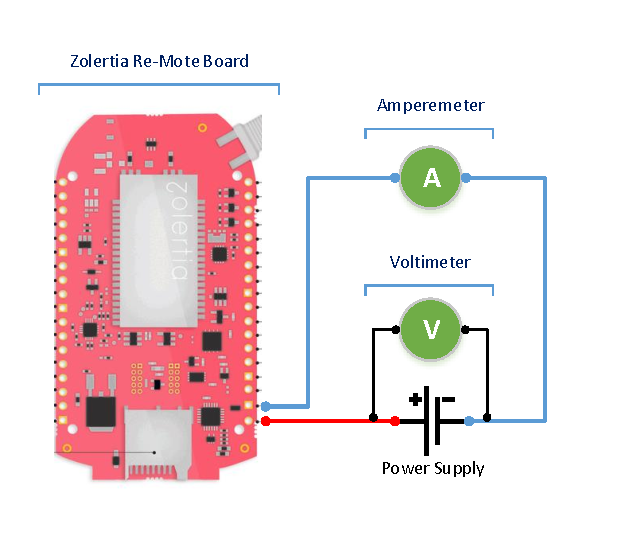
\includegraphics[width=0.65\linewidth]{figures/PowerExperiment.pdf}
  \caption{Power Consumption Experimental Setup}
  \label{fig:experimental_setup}
\end{figure}

\begin{table}
\centering
\caption{Power Consumption}
\label{tab:power_consumptions}
\begin{tabular}{|c|c|c|c|} \hline
Mode&Voltage(V)&Current(mA)&Power(W)\\ \hline
Radio ON& 9.0& 17&0.15\\ \hline
Radio OFF& 9.0& 5.2&0.05\\ 
\hline\end{tabular}
\end{table}

Knowing that the ContikiMAC \gls{RDC} protocol enables the radio to be turned off for roughly 99\% of the time\cite{Dunkels2011}, the collected data shows that our solution maintains the low-power consumptions required for \gls{IoT} environments.

\section{Propagation Delays}
The usage of an Ad-Hoc topology allows to create a network without a pre-existent infrastructure but relies on each participant node to forward data to the other elements of the network. This has impact in the time a message requires to reach its destination based on the number of hops it needs to go through. In order to measure these impacts, a study was conducted where a \gls{CoAP} Client was directly connected to the backend services in a closed room. Additionally, three \gls{CoAP} Servers were providing events to the client, routing data through each other to allow message propagation as depicted in Figure \ref{fig:message_propagation_experiment}. The experiment was conducted with a payload of 180bytes, requiring 3 packets to be sent through the network for each message. Each message was sent ten times from all the three sources. Table \ref{tab:message_propagation_results} presents the results for each server, categorizing each message group by the number of hops required for reaching its destination. The Min-Value represents the fastest message to arrive, the Max-Value represents the slowest message to arrive and the Average-Value the average of the ten attempts conducted for each server. In the case of a packet loss, each server was programmed to resend the packet up to four times, this accounts for the registered Max-Value outliers. In the case of the furtherest away server, where two hops were required for the packet to reach its destination, there were situations were even with four retransmissions the message was never successfully received by the \gls{CoAP} client. It is possible that these failures are caused by the direct exposure of the Wireless Link to a Wi-Fi Access Point located in the corridor. The impact of Wi-Fi networks is well documented in past literature \cite{Dong} and proved to cause interference and even black-out periods. We can conclude that the type of networks being used should preferably be used on locations without heavy Wi-Fi presence, but if that is not possible the network should still perform with high impacts in performance and throughput. 

\begin{figure}
  \centering
  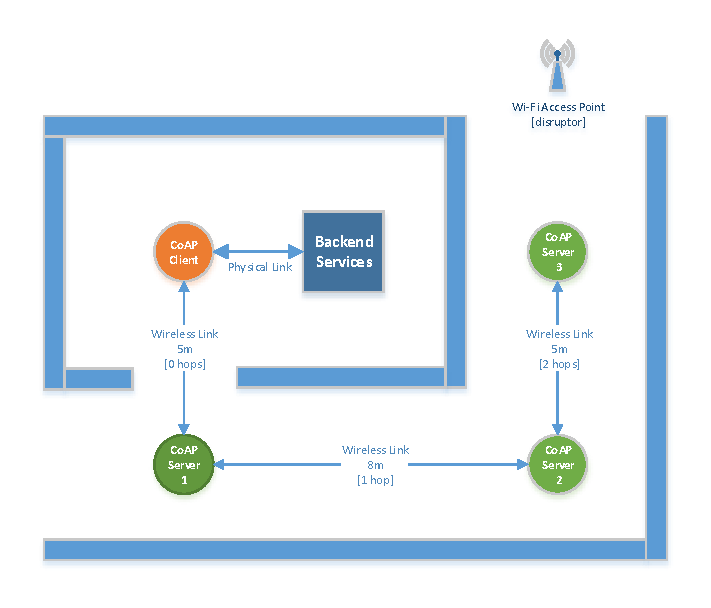
\includegraphics[width=0.8\linewidth]{figures/PropagationExperiment.pdf}
  \caption{Message Propagation Experimental Setup}
  \label{fig:message_propagation_experiment}
\end{figure}

\begin{table}
\centering
\caption{Message Propagation Results}
\label{tab:message_propagation_results}
\begin{tabular}{|c|c|c|c|} \hline
Number of Hops&Min-Value(s)&Max-Value(s)&Average-Value(s)\\ \hline
0& 0.75& 3.47&0.89\\ \hline
1& 1.50& 7.43&2.02\\ \hline
2& 12& N/A&17.9\\ 
\hline\end{tabular}
\end{table}



\section{Bootstrapping Process}
In order to evaluate our bootstrapping process we conducted an experiment on the amount of time (in seconds) required to bootstrap a new node as an indicator of the process efficiency. The process starts with the operator connecting the new device to the bootstrapper and finishes with the operator removing the device from the bootstrapper. During the process the operator needs to open the user interface, select the appropriate device and press the upload button. In the background the system will compile the source code to match the target platform, then it will erase the previous firmware and finally upload the new one. The experiment results are presented in Table \ref{tab:bootstrapping_time}. Although the apparent bootstrapping process time is 34 seconds, the process efficiency is especially important when bootstrapping multiple devices. In this case, after the first one, the user interface and target hardware will already be open and selected and the source code will already be compiled, resulting in a real time of 12 seconds. If needed, an operator could perform up to 300 bootstrapping processes in a single hour, allowing us to conclude that our solution is practical for the presented scenario.

\begin{table}
\centering
\caption{Bootstrapping Timings}
\label{tab:bootstrapping_time}
\begin{tabular}{|c|c|} \hline
Operation&Time(s)\\ \hline
Insert New Device&2\\ \hline
Open User Interface&5\\ \hline
Select Target Hardware&4\\ \hline
Compile Source Code&13\\ \hline
Erase Previous Firmware&5\\ \hline
Upload New Firmware&3\\ \hline
Remove New Device&2\\ 
\hline\end{tabular}
\end{table}

\section{Limitations}
During the development of this solution, and mainly due to compatibility issues, some limitations were raised. The most flagrant is the possibility of compromising a network node and sniffing the contents of the propagated packets. Although we are using \gls{LLSec} and this assures confidentiality, integrity, authenticity of the propagated packets while also providing authentication of the network nodes, in the event of compromising an already deployed node, the messages are cyphered and deciphered on every device, exposing the payload to the attackers. In the future a solution that protects the packets from the source all the way to the destination needs to be addressed so that the solutions can be totality secure against privacy attacks.



%!TEX root = ../dissertation.tex

\chapter{Conclusion}
\label{chapter:conclusion}
Due to the limitations of \gls{IoT} devices, achieving secure communications is not an easy task. In order to allow the deployment of battery-powered nodes, their communication model must be very efficient and consume the minimum amount of power required for operation. To achieve those requirements we started by analysing the existing protocols across the OSI layers, trying to find the best suited solutions for this type of environments. After a thorough comparison we selected a working stack of protocols but soon discovered possible breaches and attacks, especially on the network layer. These attacks were further investigated and catalogued and we found that the common flaw on the majority the attacks was the introduction of rogue nodes to the network. We then presented some possible solutions based on secure bootstrapping, the secure authentication of new nodes when joining a network.\\
Once a working protocol stack was assembled, possible attacks and mitigation strategies were defined, and we proposed our solution based on a Smart Campus scenario. This solution is focused on providing the joining devices all the secure credentials required for a secure bootstrapping before the deploy on the field, so that when they start the operation phase no additional credentials need to be fetched, implying that no additional energy is spent on configuration.\\
The achieved solution was then evaluated and the results confirm that it is suitable for operation since it fits the hardware commonly used in the \gls{IoT} while maintaining a low power consumption. Also, experiments showed that the bootstrapping process can be done by users without inner knowledge of the system and without requiring much time to complete. Furthermore, although the network faces severe disruption in the presence of Wi-Fi networks, it can still operate under stress with diminished performance.

\section{Future Work}

Although the achieved solution is working and fulfilling the proposed objectives there is room for improvement and additional work. As discussed in Section \ref{sec:attack_analysis}, an attacker could try to introduce himself to the network by \emph{stealing the network credentials} from a deployed device. The mitigations strategies for this attack can be either software based,  assuring that secure memory areas cannot be copied to external locations, or hardware based, certain integrated circuits assure the stored information cannot be read from them \cite{Lesjak2014}. Although they have not been address in this system as we believe they are out of the scope of this project and more related to other computer science fields, they are still important and need to be addressed for increasing the security of the system globally.\par 
To further protect the network against this attack, future changes can also be performed on the management station. An improvement would be to \emph{keep track of the connected devices} and fire alerts when two devices with the same identifier started operating. Since there cannot be two devices with the exact same properties, this situation would mean that the firmware of an authorized node was somehow cloned into a rogue device.\par
Regarding the used \emph{hardware and interfacing} capabilities, one could attempt, in order to avoid the necessity of physical connections, to resort to the always required 802.15.4 radio as the way of sending the custom firmware to the new device. This would need to be done on a secure environment so that the firmware could not be sniffed by any attacker and from that firmware be able to steal the network credentials, but would reduce the time and hardware connections required for flashing a new device. Although our goal was never a massive deployment, but scenarios with the dimension of a Smart Campus, this question loses some relevance. However it is still important to this about this system as possibly being used on a large scale enterprise solution and to that extent this issue needs to be addressed.\par
Thinking about \emph{scalability}, due to the small amount of physical devices available for testing, we never constructed a network larger than four nodes, meaning the capabilities of the system under heavy usage were not tested. This is important and needs to be studied before thinking about deploying this system on a large scale. To achieve that, one could try, in the future, to integrate this system with the IoT-LAB \footnote{https://www.iot-lab.info/} large scale infrastructure facility suitable for testing small wireless sensor devices and heterogeneous communicating objects. If such integration could be achieved, the system could be tested with dozens of nodes on real hardware devices.





\bibliographystyle{ieeetr}
\addcontentsline{toc}{chapter}{Bibliography}
\bibliography{bibliography/references}

% Appendix
\appendix
%!TEX root = ../dissertation.tex

% Appendix chapters entry point
% Include the chapters below

%!TEX root = ../dissertation.tex

\chapter{Appendix chapter}
\label{appendix:appendix_chapter}



% Glossary and Acronym List
\if\includeGlossary 1
\printglossary
\fi

% Back Cover
\pagenumbering{gobble}
\NewPage

\end{document}
